%\documentclass[conference, onecolumn]{IEEEtran}
\documentclass[11pt]{article}
\usepackage[a4paper,left=3cm,right=3cm,top=3cm,bottom=3.75cm,footskip=1.5cm,headsep=1cm]{geometry}

%\IEEEoverridecommandlockouts
% The preceding line is only needed to identify funding in the first footnote. If that is unneeded, please comment it out.
\usepackage{cite}
\usepackage{listings}
\usepackage{tikz}
\usepackage{amsmath,amssymb,amsfonts}
\usepackage{algorithmic}
\usepackage{graphicx}
\usepackage{textcomp}
\usepackage{xcolor}
\usepackage{url}
\usepackage{float}
\usepackage{MnSymbol}

\renewcommand{\figurename}{Abbildung}

\def\BibTeX{{\rm B\kern-.05em{\sc i\kern-.025em b}\kern-.08em
    T\kern-.1667em\lower.7ex\hbox{E}\kern-.125emX}}

\newcommand\YAMLcolonstyle{\color{red}\mdseries}
\newcommand\YAMLkeystyle{\color{black}\bfseries}
\newcommand\YAMLvaluestyle{\color{blue}\mdseries}

\lstset{prebreak=\raisebox{0ex}[0ex][0ex]
        {\ensuremath{\rhookswarrow}}}
\lstset{postbreak=\raisebox{0ex}[0ex][0ex]
        {\ensuremath{\rcurvearrowse\space}}}
\lstset{breaklines=true, breakatwhitespace=true}
\lstset{numbers=left, numberstyle=\scriptsize}

\definecolor{maroon}{rgb}{0.5,0,0}
\definecolor{darkgreen}{rgb}{0,0.5,0}
\lstdefinelanguage{XML}
{
	basicstyle=\ttfamily,
	morestring=[s]{"}{"},
	morecomment=[s]{?}{?},
	morecomment=[s]{!--}{--},
	commentstyle=\color{darkgreen},
	moredelim=[s][\color{black}]{>}{<},
	moredelim=[s][\color{red}]{\ }{=},
	stringstyle=\color{blue},
	identifierstyle=\color{maroon}
}

\makeatletter

% here is a macro expanding to the name of the language
% (handy if you decide to change it further down the road)
\newcommand\language@yaml{yaml}

\expandafter\expandafter\expandafter\lstdefinelanguage
\expandafter{\language@yaml}
{
  keywords={true,false,null,y,n},
  keywordstyle=\color{darkgray}\bfseries,
  basicstyle=\YAMLkeystyle,                                 % assuming a key comes first
  sensitive=false,
  comment=[l]{\#},
  morecomment=[s]{/*}{*/},
  commentstyle=\color{purple}\ttfamily,
  stringstyle=\YAMLvaluestyle\ttfamily,
  moredelim=[l][\color{orange}]{\&},
  moredelim=[l][\color{magenta}]{*},
  moredelim=**[il][\YAMLcolonstyle{:}\YAMLvaluestyle]{:},   % switch to value style at :
  morestring=[b]',
  morestring=[b]",
  literate =    {---}{{\ProcessThreeDashes}}3
                {>}{{\textcolor{red}\textgreater}}1     
                {|}{{\textcolor{red}\textbar}}1 
                {\ -\ }{{\mdseries\ -\ }}3,
}

% switch to key style at EOL
\lst@AddToHook{EveryLine}{\ifx\lst@language\language@yaml\YAMLkeystyle\fi}
\makeatother

\newcommand\ProcessThreeDashes{\llap{\color{cyan}\mdseries-{-}-}}

\begin{document}

\title{Projektarbeit: Unmanned Surface Vehicle}

%\author{\IEEEauthorblockN{Josephine Brauer}
%\\
%\and
%\IEEEauthorblockN{Kilian Schweppe}
%\\
%}
\author{Josephine Brauer \and Kilian Schweppe}

\maketitle

\begin{abstract}
In dieser Projektarbeit wurde ein im Rahmen einer Bachelorarbeit entwickeltes Oberflächenfahrzeug für Wasserexploration in Rettungsszenarien durch Software ergänzt, die es ermöglicht, autonom ein Gewässer abzufahren und dabei die Wassertiefe zu erfassen.\\
Die notwendigen Funktionalitäten wurden in Python unter Nutzung von ROS und des von ROS bereitgestellten Navigation Stacks implementiert. Um die Funktionsweise testen zu können, wurde außerdem eine Simulation des Bootes auf Basis eines bestehenden Simulators erstellt.\\
Die richtige Funktionsweise des Bootes wurde im Simulator getestet.
\end{abstract}

\section{Einleitung}
Mit einem Anstieg der Anzahl der Naturkatastrophen und ihren verursachten Kosten in den letzten Jahrzehnten\cite{kellenberg} nimmt auch die Notwendigkeit zu, Möglichkeiten für die Verhinderung und Bewältigung von Katastrophen zu finden. Auch die Robotik bietet immer wieder Lösungen, die im Katastrophenschutz eingesetzt werden können. Dabei haben Unbemannte Fahrzeuge insbesondere zur Erfassung von Daten ein großes Potenzial \cite{surveyDisasterRobotics}.

Sie können Einsatzkräfte in unzugänglichen oder gefährlichen Umgebungen ersetzen \cite{bellingham}, welche damit sowohl geschützt, als auch anderen Aufgaben zugeteilt werden können. Durch die potenziell geringe Größe und Lautstärke der Fahrzeuge können auch Gebiete erfasst werden, die sonst entweder nicht zugänglich wären, oder unter größeren Eingriffen in die Natur leiden könnten, wie zum Beispiel Naturschutzgebiete. Mit unseren 201 Naturschutzgebieten in Schleswig-Holstein, und weiteren in Planung \cite{Naturschutz}, hat dieses Thema auch in unserer Region eine besondere Relevanz.

Besonders für lang andauernde Aufgaben und in Regionen, in denen man damit rechnen muss, nicht immer mit dem Fahrzeug kommunizieren zu können, kann es sinnvoll sein, diese Fahrzeuge nicht nur unbemannt, sondern auch autonom zu gestalten, da das Fahrzeug so nicht durchgehend angesteuert werden muss.

In Hinsicht auf Katastrophen spielt der Schutz vor Hochwasser in Schleswig-Holstein eine besondere Rolle, da laut der Landesregierung etwa ein Viertel der Landesfläche und mehr als 350.000 Menschen durch Sturmfluten gefährdet sind\cite{Hochwasser}. In Lübeck und Umgebung sind vor allem Flusshochwasser ein Problem (s. Abbildung \ref{Hochwassergefahrenkarte}). Hier könnten Unbemannte Wasserfahrzeuge zum Beispiel durch frühzeitiges Erkennen von Deichbrüchen helfen. Die denkbaren Anwendungsfelder sind allerdings nicht nur auf den Schutz vor Schäden durch unsere Gewässer begrenzt, vielmehr könnten sie auch den Schutz unserer Gewässer selbst abdecken, etwa durch Identifikation von Verschmutzungen und ihrer Quellen.

\begin{figure}[h]
	\centering
	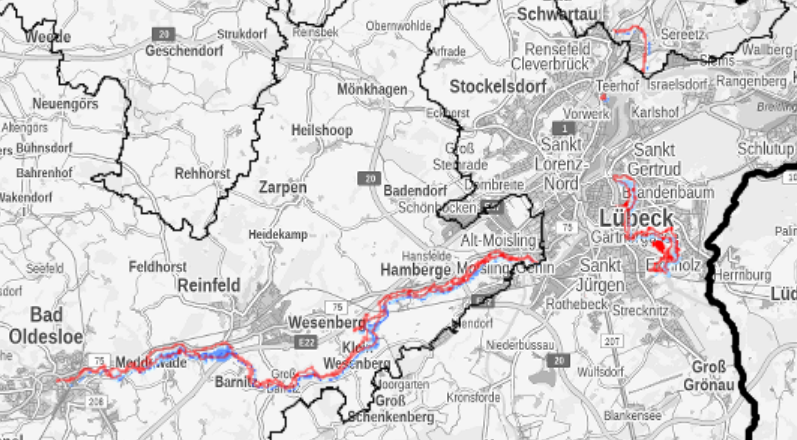
\includegraphics[width=0.8\linewidth]{Hochwasserrisiko.png}
	\caption{Hochwassergefahrenkarte für Hochwasser mit hoher Wahrscheinlichkeit, Quelle: \protect\url{http://zebis.landsh.de/webauswertung/index.xhtml} ©GeoBasis-DE/LVermGeo SH, BKG}
	\label{Hochwassergefahrenkarte}
\end{figure}

Für den Einsatz im und auf dem Wasser sind unter anderem Unbemannte Unterwasserfahrzeuge (UUVs) und Unbemannte Oberflächenfahrzeuge (USVs) möglich \cite{surveyDisasterRobotics}. USVs haben dabei den Vorteil, mehr Sensoren über eine längere Zeitdauer tragen zu können und damit mehr verschiedene Messungen gleichzeitig über einen längeren Zeitraum durchführen zu können, wobei sowohl Messungen an der Oberfläche als auch im Wasser möglich sind \cite{coley2015}. Trotzdem wird ihnen bis jetzt in der Literatur weniger Beachtung gewidmet, als den Unbemannten Unterwasser Fahrzeugen \cite{surveyDisasterRobotics}. \newline

Aus den genannten Gründen erscheint uns die Entwicklung autonomer USVs, die für vielfältige Szenarien im Bereich der Rettungsrobotik ausgerüstet sind, sinnvoll. In dieser Arbeit sollen dafür erste notwendige Schritte erfolgen, indem ein im Rahmen einer Bachelorarbeit entwickeltes Oberflächenfahrzeug für Wasserexploration in Rettungsszenarien durch Software ergänzt wird, die das autonome Befahren eines Gewässers ermöglicht. Da auf dem USV bereits ROS installiert und genutzt wird, liegt es nahe, vom von ROS bereitgestellten Navigation Stack \footnote{\url{https://github.com/ros-planning/navigation}} Gebrauch zu machen. Dieser bietet viele nützliche Funktionalitäten -unter anderem werden mehrere globale und lokale Planer bereitgestellt- für die autonome Navigation von mobilen Robotern \cite{zheng2019ros}. Es gibt sowohl ein Tutorial von ROS \footnote{\url{http://wiki.ros.org/navigation/Tutorials}}, als auch einige andere Quellen (z.B. \cite{zheng2019ros}), die sich mit der Benutzung des Navigation Stacks auseinandersetzen. Auf GitHub wurde das Projekt bis heute etwa 1400 Mal geforkt (Stand 08.03.2021). Das spricht für die Popularität des Navigation Stacks, weshalb angenommen werden kann, dass die Verwendung des Navigation Stacks die Verständlichkeit des Projekts auch für Außenstehende verbessert.\\

Des Weiteren wollen wir ein Anwendungsszenario, das Erfassen der Wassertiefe, implementieren und testen. Die Aufzeichnung der Wassertiefe könnte zum Beispiel hilfreich bei der Suche nach vermissten Personen oder Gegenständen, wie zum Beispiel Autos, sein.\\

Um die Funktionsweise des Bootes testen zu können, ohne Gefahr zu laufen, das Boot auf dem Wasser zu verlieren, und zukünftigen Gruppen die Arbeit mit dem Boot zu erleichtern, soll außerdem eine Simulation des Bootes auf Basis eines bestehenden Simulators erstellt werden.

\section{Methoden}

Auf Basis unserer Zielstellung haben wir mehrere Arbeitspakete identifiziert, auf deren Durchführung im Folgenden eingegangen werden soll:
\begin{enumerate}
	\item Einarbeitung in die Simulationsumgebung
	\item Simulation der Sensoren des Bootes
	\item Simulation der Ausgaben des Bootes
	\item Implementierung der Schnittstellen zum Navigation Stack
	\item Navigation zu Wegpunkten
	\item Vermeidung unerwarteter Hindernisse
	\item Erstellung von Wegpunkten auf Basis der Karte
	\item Erfassung der Wassertiefe und Eintragung in Karte
	\item Ignorieren unerwartet nicht anfahrbarer Zielpunkte
	\item Homing Verhalten

\end{enumerate}

\subsection{Einarbeitung in die Simulationsumgebung}
Als Simulationsumgebung wurde uns \textit{Simulated enviroment for Unmanned Surface Vehicles}\footnote{\url{https://github.com/disaster-robotics-proalertas/usv_sim_lsa}} vorgeschlagen. Das Besondere an diesem Simulator ist, dass dieser Umwelteinflüsse wie die Wasseroberfläche inklusive Wellen, die Strömung des Gewässers und den Wind simuliert, weshalb besonders realistische Szenarien gestaltet werden können. Außerdem handelt es sich um eine Gazebo-Simulation, weshalb die Nodes, die später auf dem echten Boot laufen sollen, fast unverändert in der Simulation verwendet werden können. Des Weiteren werden mehrere Boot-Modelle bereitgestellt, die gut als Grundlage für ein eigenes Szenario genutzt werden können\cite{paravisi2019}.\\

Da das Projekt nicht optimal dokumentiert ist, hat die Einarbeitung in den Simulator mehr Zeit in Anspruch genommen, als ursprünglich gedacht.\\
Der Master-Branch des Simulators benutzt ROS Kinetic. Da auf dem USV aber momentan ROS Melodic läuft und darüber hinaus Kinetic nach April 2021 nicht mehr von ROS unterstützt wird \cite{rosdistros}, hielten wir es für sinnvoll, zu versuchen, den Simulator auf ROS Melodic laufen zu lassen. Obwohl das Projekt über einen dafür vorgesehenen Branch\footnote{\url{https://github.com/disaster-robotics-proalertas/usv_sim_lsa/tree/master-melodic}} verfügt, mussten wir dieses Vorhaben letztendlich aus Zeitgründen und aufgrund von für uns nicht lokalisierbaren Problemen abbrechen und mit Kinetic weiterarbeiten.\newline

Der Übersichtlichkeit halber wollen wir hier einen Überblick über die Bestandteile geben, die für unser Projekt angepasst wurden:\\
Die Simulationsumgebung stellt 4 verschiedene Boot-Modelle bereit: ein Airboot, ein Differentialboot, ein Ruderboot und ein Segelboot \cite{paravisi2019}. Wir haben das Differentialboot-Modell als Grundlage für unser Modell genommen, da es sich bei unserem USV ebenfalls um ein Boot mit 2 Motoren am Heck (s. Abbildung \ref{boot}) handelt. Wir haben 2 Dateien identifiziert, die das Boot modellieren: \texttt{diffboat.xacro} (modelliert unter anderem die Motoren) und \texttt{boat\_subdivided\_validated.xacro} (modelliert unter anderem Sensoren). Diese Dateien wurden als Grundlage genutzt, um unser Boot zu modellieren.

Die Szenarien befinden sich im Ordner \texttt{scenes}. Durch die Bearbeitung der XML-Dateien kann man z.B. die Anzahl und Positionen der Boote und Bojen, die Position und Art des Terrains und die Position der Kamera anpassen.\\
Ebenfalls hilfreich für die Erstellung neuer Szenarien sind die launch-Dateien in den folgenden Ordnern:

\begin{itemize}
	\item \texttt{usv\_sim\_lsa/usv\_sim/launch/scenarios\_launchs/}: hier kann man unter anderem die zu verwendende Welt angeben.
	\item \texttt{usv\_sim\_lsa/usv\_sim/launch/models/}: hier werden unter anderem die Nodes gestartet, die "auf dem Boot laufen", also zum Beispiel Nodes, die Transformationen publishen oder die Bewegungen des Bootes kontrollieren.
\end{itemize}

\subsection{Simulation der Sensoren des Bootes}

Auf dem Boot sind mehrere Sensoren zu finden:

\begin{itemize}
	\item ein GPS-Gerät
	\item ein Kompass
	\item ein Ultraschallsensor für die Wassertiefe
	\item ein Ultraschallsensor für die Erkennung von Hindernissen am Bug
	\item eine 360°-Kamera
	\item ein Temperatursensor
\end{itemize}

Darüber hinaus verfügt das Boot noch über 2 Motoren für die Fortbewegung und eine 4G/WIFI-Anbindung zur Kommunikation (s. Abbildung \ref{boot}).\\

\begin{figure}[h]
    \centering
	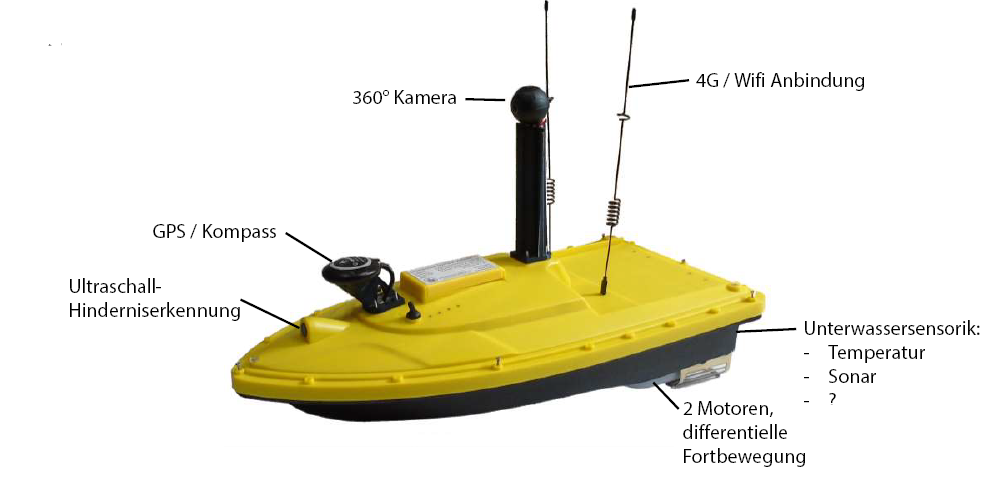
\includegraphics[width=0.9\linewidth]{boot.png}
	\caption{Sensoren und Aktuatoren des Bootes}
	\label{boot}
\end{figure}

Detaillierte Informationen zu allen Sensoren und Aktuatoren des Bootes und den erwarteten Ein- und Ausgabewerten lassen sich im zugehörigen GitHub-Projekt finden \footnote{\url{https://github.com/NRottmann/UzL_USV/}}.
Für die Implementierung unseres Szenarios in der Simulation benötigten wir die GPS-, Kompass- und Ultraschalldaten und die Motoren. Deshalb haben wir ein GPS-Modul und zwei Ultraschall-Sensoren zum Differentialboot-Modell des Simulators hinzugefügt. Außerdem haben wir das Modell durch eine IMU zur Simulierung der Orientierung ergänzt. Dazu haben wir die \texttt{GazeboRosGps}, \texttt{GazeboRosImu} und \texttt{GazeboRosSonar} Plugins aus dem Paket \texttt{hector\_gazebo\_plugins}  \footnote{\url{https://github.com/tu-darmstadt-ros-pkg/hector_gazebo}} verwendet.

%\begin{figure}
%	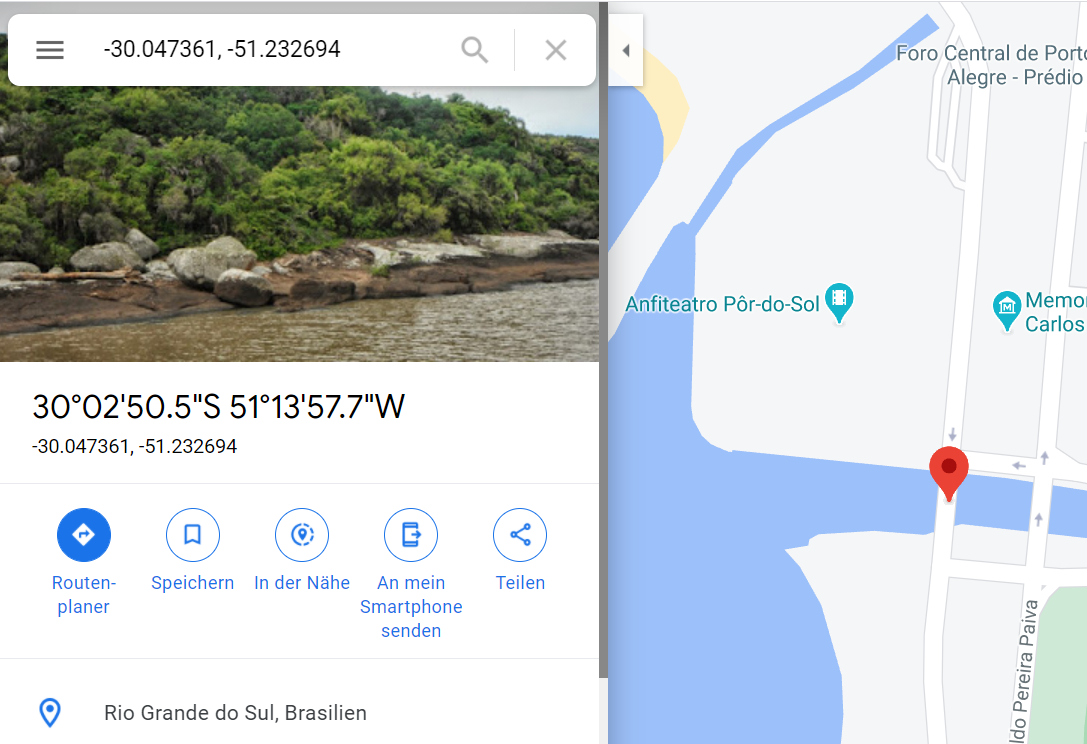
\includegraphics[width=\linewidth]{reference.png}
%	\caption{Referenzkoordinaten}
%	\label{reference}
%\end{figure}

Da wir für unser Szenario weitestgehend das \texttt{diffboat\_scenario1} übernommen haben (das einen Ausschnitt von Porto Alegre, Brasilien, nahe der Mündung des Dilúvio zeigt \cite{paravisi2019}), haben wir die GPS-Koordinaten eines markanten Punktes im Szenario bestimmt und als Referenzkoordinaten für die Simulierung der GPS-Daten gewählt.

\subsection{Simulation der Ausgaben des Bootes}

Nachdem wir die notwendigen Daten simuliert haben, die auch das echte Boot sammelt, wollten wir die Daten auch in derselben Form ausgeben, wie es das USV bereits tut. Dafür haben wir die notwendigen Topics und deren Inhalt bestimmt:

\begin{itemize}
	\item \texttt{range\_front}: Daten des vorderen Sonars
	\item \texttt{range\_depth}: Daten des unteren Sonars
	\item \texttt{velocity}: Geschwindigkeit des Bootes in Bewegungsrichtung
	\item \texttt{heading}: unterteilt sich in \texttt{gps\_heading}: die Bewegunsrichtung des Bootes und \texttt{mag\_heading}: die Orientierung des Bootes
	\item \texttt{gps}: GPS-Koordinaten des Bootes
	\item \texttt{safety}: Informationen zu Batteriestand, Spannung, Strom, Ladung und ob sich Wasser innerhalb des Bootes befindet
\end{itemize}
\texttt{range\_front}, \texttt{range\_depth} und \texttt{gps} konnten dabei als Parameter im jeweiligen XML-Element gegeben werden. Für das Publishen von \texttt{velocity} und \texttt{heading} haben wir die Simulationsumgebung durch Skripte ergänzt:
Die Geschwindigkeit des Bootes in Bewegungsrichtung, \texttt{velocity}, berechnen wir in \texttt{vel\_pub} über die Formel:

\begin{equation}
v = \sqrt{x^2+y^2}
\end{equation}

Dabei ist x die Geschwindigkeit in x-Richtung und y die Geschwindigkeit in y-Richtung.\\
Nach ROS-Konvention soll die x-Achse Richtung Osten und die y-Achse Richtung Norden zeigen \cite{REP105}. Dies wird in der Simulationsumgebung ebenfalls eingehalten, also haben wir uns bei der Implementierung an dieser Konvention auch orientiert. Wenn im Folgenden von x- oder y-Achse die Rede ist, sei damit auch immer die Achse in Richtung Osten oder Norden gemeint.\\
Deshalb können wir die beiden benötigten Werte aus dem Topic \texttt{gps/velocity} auslesen, welches vom simulierten GPS-Modul gepublisht wird.\\
Für \texttt{heading} bestimmen wir in \texttt{heading\_pub} die beiden Komponenten \texttt{gps\_heading} und \texttt{mag\_heading} einzeln:\\
Über 
\begin{equation}
	atan2(x,y) 	
\end{equation}
(wobei wieder x die Geschwindigkeit in x-Richtung und y die Geschwindigkeit in y-Richtung ist) bestimmen wir das \texttt{gps\_heading}, also die Bewegungsrichtung nach GPS. \\
Aus der Komponente \texttt{orientation} der simulierten IMU kann durch Umwandlung der ausgegebenen Quaternion in Euler-Winkel das \texttt{mag\_heading} bestimmt werden.\\
Beide Winkelangaben haben wir noch so angepasst, dass statt bei einer Orientierung Richtung Osten, bei einer Orientierung Richtung Norden 0° vorliegen. Beide Werte werden danach auf das Topic \texttt{heading} gepublisht. Einen Überblick der zur Simulierung der Ausgaben des Bootes genutzten Nodes findet sich in Abbildung \ref{output-sim-nodes}.\\

\begin{figure}[h]
	\centering
	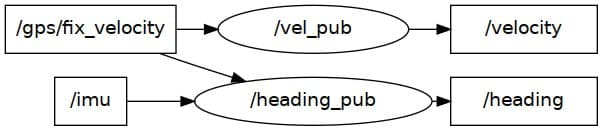
\includegraphics[width=0.7\linewidth]{simulation-nodes}
	\caption{Nodes zur Simulierung der Ausgaben des Bootes}
	\label{output-sim-nodes}
\end{figure}
Außerdem haben wir ein Skript \texttt{safety\_pub} hinzugefügt, dass den Batteriestand und den Wassersensor modelliert und auf das Topic \texttt{safety} publisht. Dabei wird momentan ein linearer Abfall des Batteriestandes und eine Akkulaufzeit von 1h angenommen. Für den Wassersensor haben wir eine gewisse Wahrscheinlichkeit ausgewählt, mit der der Wert des Sensors auf 1 springt. Beide Parameter lassen sich in der Datei \texttt{spawn\_rescue\_robotics\_boat.launch} anpassen:

\begin{lstlisting}[language=xml]
<node name="safety_pub" pkg="usv_uzl" type="safety_pub.py">
    <param name="battery_duration" value="60"/>
    <param name="water_probability" value="0.001"/>
</node>
\end{lstlisting}

Die Werte für Spannung, Strom und Ladung modellieren wir nicht, da sie für unser Szenario nicht relevant waren.
Außerdem haben wir auf das Publishen der folgenden Topics vorerst verzichtet, da diese für unseren Anwendungsfall nicht notwendig waren:
\begin{itemize}
	\item \texttt{mag}
	\item \texttt{temperature}
\end{itemize}

\subsection{Implementierung der Schnittstellen zum Navigation Stack}
Der Navigation Stack nutzt Odometrie- und Sensordaten, um Kommandos bezüglich der Geschwindigkeit an einen mobilen Roboter geben zu können, um einen bestimmte Zielkoordinaten zu erreichen. Damit dies möglich ist, müssen auf dem Roboter erst bestimmte Schnittstellen implementiert werden\cite{NavWiki}. In Abbildung \ref{nav} zu kann man mehrere Topics erkennen, die als Schnittstellen zwischen Roboter und Navigation Stack fungieren:
\begin{itemize}
	\item \texttt{tf}
	\item \texttt{odom}
	\item \texttt{map}
	\item \texttt{move\_base\_simple/goal}
	\item Sensor Topics des Formates LaserScan oder PointCloud
	\item \texttt{cmd\_vel}
\end{itemize}
Im Folgenden soll es darum gehen, wie wir die Werte der Topics generiert bzw. verarbeitet haben. Da wir in der Simulation dieselben Ausgabeschnittstellen erzeugt haben, wie wir sie auf dem echten Boot vorliegen haben werden, sollten die Implementationen der Schnittstellen gut auf das echte Boot übertragbar sein.

\begin{figure}[h]
	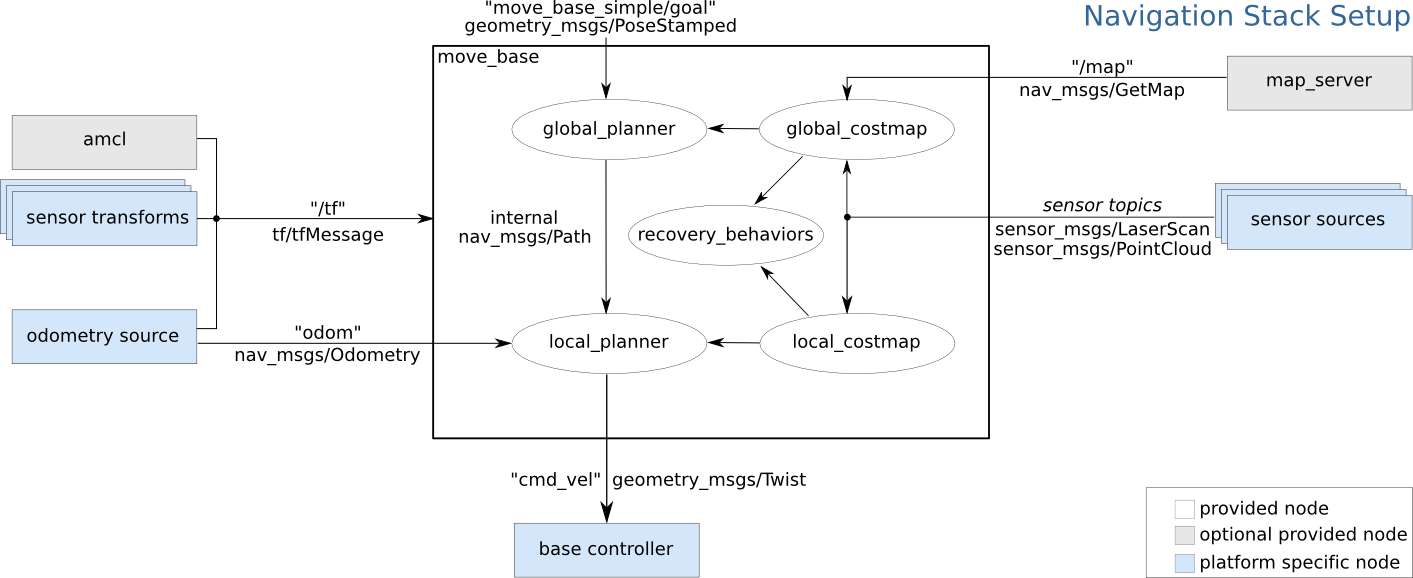
\includegraphics[width=\linewidth]{overview_tf.png}
	\caption{Robot Setup Navigation Stack (Quelle: http://wiki.ros.org/navigation/Tutorials/RobotSetup (Stand: 2018-07-19 02:43:42))}
	\label{nav}
\end{figure}

\subsubsection{tf}

\begin{figure}[h]
	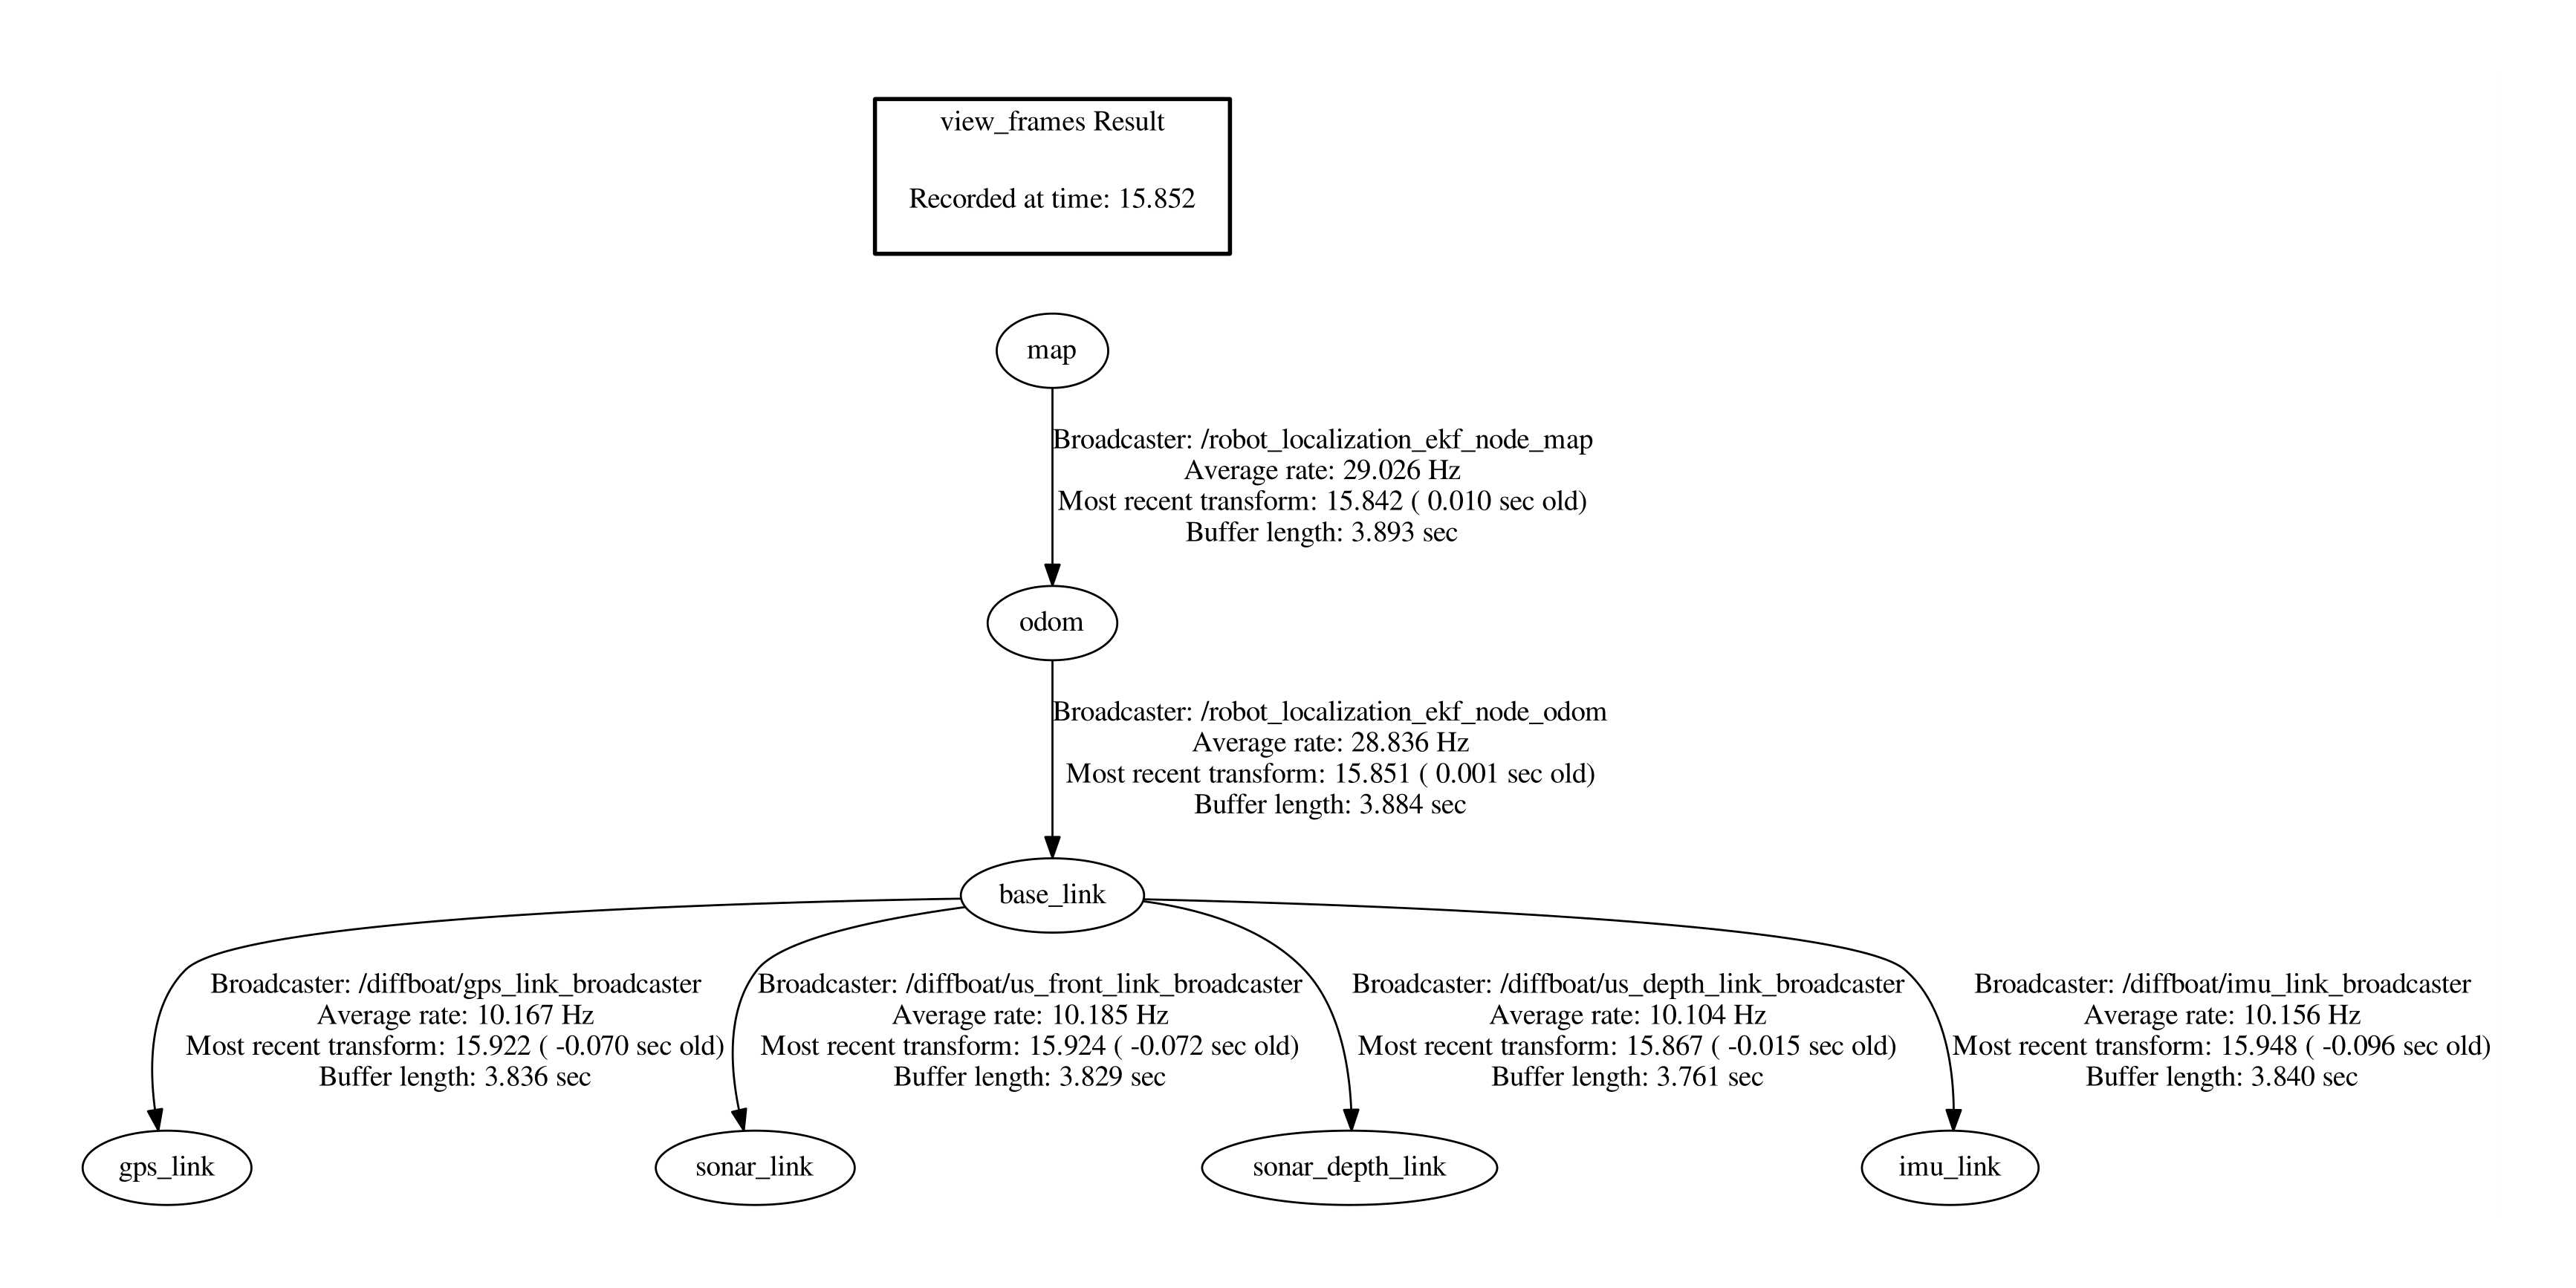
\includegraphics[width=\linewidth]{frames.png}
	\caption{Tf Tree}
	\label{frames}
\end{figure}

Der Navigation Stack benötigt 2 Transformationen um zu funktionieren, eine vom \texttt{map}-Frame zum \texttt{odom}-Frame und eine vom \texttt{odom}-Frame zum \texttt{base\_link}-Frame. Wie in \texttt{REP-105} \cite{REP105} spezifiziert, ist das \texttt{map}-Frame ein statisches Weltkoordinatensystem, welches die Position des Bootes in kartesischen Koordinaten auf der Karte darstellt.  Das \texttt{odom}-Frame ist ebenfalls ein statisches Koordinatensystem, in dem durch Auswertung der Odometrie die theoretische Position des Bootes bestimmt wird, welche zwar von der echten Position stark abweichen kann, aber dennoch eine genauere Lokalisierung ermöglicht.

Für die Erstellung dieser Transformationen setzen wir das \texttt{robot\_localization} \footnote{\url{http://wiki.ros.org/robot_localization}} Paket ein, welches die nötigen Transformationen bereits zur Verfügung stellt, GPS Koordinaten in Weltkoordinaten umrechnet und Sensorinformationen mit einem Kalman-Filter zusammenfügt \cite{MooreStouchKeneralizedEkf2014}. Der reultierende Transformations-Tree einschließlich der statischen Transformationen ist in Abbildung \ref{frames} zu sehen.\\

Für die Transformation vom \texttt{odom}- zum \texttt{base\_link}-Frame nutzen wir den \texttt{ekf\_localization\_node}. Dieser kann Messages der Form:
\begin{itemize}
	\item Odom
	\item Imu
	\item Pose
	\item Twist
\end{itemize}
verwerten.
In unserem Fall wird die Geschwindigkeit in Bewegungsrichtung (\texttt{velocity}) für die Berechnung einer Odom-Message verwendet.
Außerdem benutzen wir \texttt{mag\_heading} und die aus der Ableitung von \texttt{mag\_heading} berechnete Winkelgeschwindigkeit zur Erzeugung einer IMU-Message.\\
Obwohl wir bei der Orientierung nach Kompass (\texttt{mag\_heading}) in Bewegung eine ungenauere Näherung an die Bewegungsrichtung erwarten, als die Orientierung nach GPS (\texttt{gps\_heading}) liefern würde, haben wir uns für die Verwendung von \texttt{mag\_heading} entschieden, da für die Berechnung der Odometrie kontinuierliche Daten erwartet werden \cite{REP105}. Bei \texttt{gps\_heading} kann es im Gegensatz zu \texttt{mag\_heading} zu diskreten Sprüngen kommen.\\

Für die Lokalisierung im Weltkoordinatensystem (also im \texttt{map}-Frame) wurde ebenfalls ein \texttt{ekf\_localization\_node} aufgesetzt. Dieser bekommt eine Odom-Message von einem \texttt{navsat\_transform\_node} \footnote{\url{http://docs.ros.org/en/noetic/api/robot_localization/html/navsat_transform_node.html}}, der die Daten vom Topic \texttt{gps} entsprechend umwandelt. Eine Übersicht der genutzten Nodes ist in Abbildung \ref{localization-overview} zu sehen.

\begin{figure}[h]
	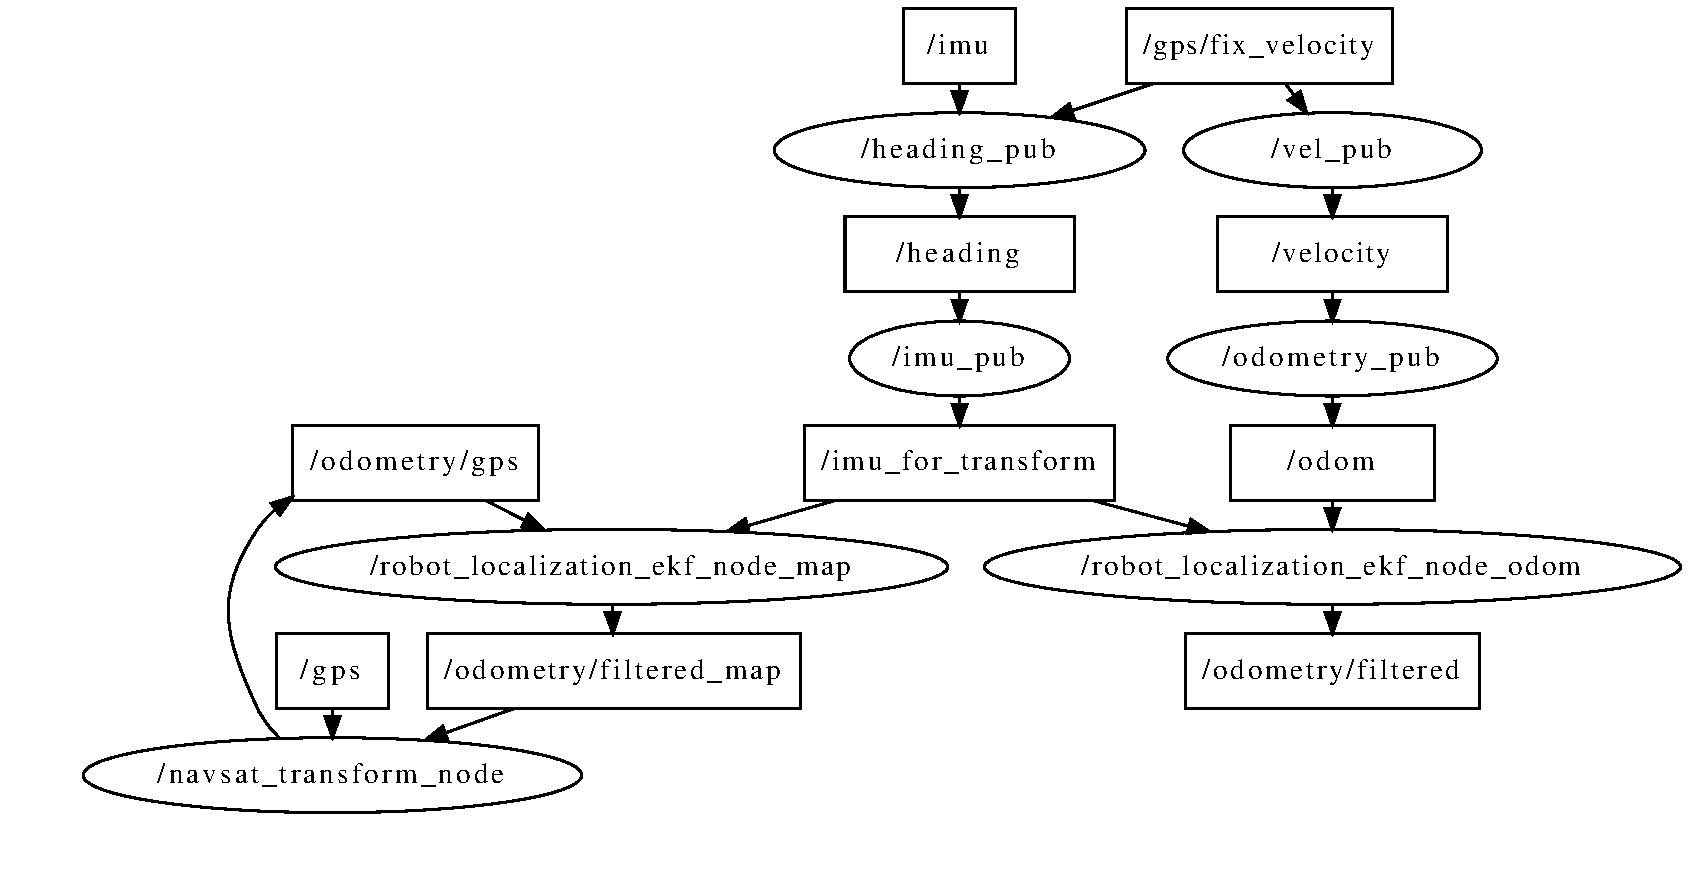
\includegraphics[width=\linewidth]{localization-nodes}
	\caption{Localization Nodes}
	\label{localization-overview}
\end{figure}

\subsubsection{odom}

Die von dem Navigation Stack genutzte Odometrie kommt aus dem Topic \texttt{/odometry/filtered\_map}, welches vom Node \texttt{robot\_localization\_ekf\_node\_map} ausgegeben wird.

\subsubsection{map}

Für den Map Server haben wir eine schwarz-weiß Karte der in der Simulation dargestellten Region (\ref{diluvio}) erstellt. Dabei stellen weiße Regionen befahrbare und schwarze unbefahrbare Gebiete dar.

\begin{figure}[h]
	\centering
	
\includegraphics[width=0.7\linewidth]{diluvio.jpg}
	\caption{Simulierte Region, © OpenStreetMap-Mitwirkende}
	\label{diluvio}
\end{figure}

Wichtige Informationen über die Karte, wie die Anzahl der Meter pro Pixel, sowie die Platzierung der linken unteren Ecke in der Simulationsumgebung haben wir berechnet und in einer yaml-Datei gespeichert.

\subsubsection{move\_base\_simple/goal} \label{goal}
Statt direkt auf das Topic \texttt{move\_base\_simple/goal} zu publishen, benutzen wir die \texttt{actionlib} API \footnote{\url{http://wiki.ros.org/actionlib}}. Diese hat den Vorteil, dass man direkt eine Callback-Methode übergeben kann, die aufgerufen wird, wenn das übergebene Ziel erreicht wurde. Das ist für uns besonders nützlich, da wir so die Messwerte an bestimmten Positionen leicht speichern können (s. \ref{measurements}).

\subsubsection{Sensor Topics} \label{sensor-topics}
Statt die normalerweise vom Navigation Stack genutzten \texttt{LaserScan}-Topics und \texttt{PointCloud}-Topics zu nutzen, um Hindernisse in die globale und lokale Costmap eintragen zu können und so auch unerwarteten Hindernissen ausweichen zu können, nutzen wir das \texttt{range\_sensor\_layer}-Plugin \footnote{\url{http://wiki.ros.org/range_sensor_layer}}, um die Daten des vorderen Ultraschallsensors direkt verwenden zu können. Im Vergleich zur Nutzung der Ultraschall-Daten zur Erstellung einer \texttt{PointCloud}-Message, lieferte diese Herangehensweise die besseren Resultate, da mit der \texttt{PointCloud}-Message Hindernisse in den Tests häufig nicht gut umfahren wurden.

\subsubsection{cmd\_vel} \label{cmd}

Die Werte aus \texttt{cmd\_vel} werden in dem Skript \texttt{boat\_diff\_vel\_ctrl} in lineare Geschwindigkeit und Winkelgeschwindigkeit aufgeteilt. Aus der Differenz dieser und der aktuellen linearen und Winkelgeschwindigkeit aus dem Topic \texttt{/odometry/filtered\_map} werden dann je Regeldifferenzen für die lineare und Winkelgeschwindigkeit berechnet, welche danach genutzt werden, um mit Hilfe zweier PID-Regler die ausgeregelten Geschwindigkeiten zu errechnen, die auf die Motoren geschrieben werden.

\subsection{Navigation zu Wegpunkten}

Die tatsächliche Navigation zu den Wegpunkten ist nach Implementierung der Schnittstellen Aufgabe des Navigation Stacks (durch das Publishen des Topics \texttt{cmd\_vel}).\\
In Testläufen mit reiner Weiterleitung der \texttt{cmd\_vel}-Werte auf die Motoren konnte kein sicheres Anfahren der Zielpunkte erreicht werden, obwohl mehrere lokale Planer mit unterschiedlichen Parametern ausprobiert wurden. Der stabilste Planer schien der \texttt{teb\_local\_planner} \footnote{\url{http://wiki.ros.org/teb_local_planner}} zu sein, weshalb wir uns letztendlich für diesen entschieden haben. 
Wir vermuteten als Grund für die mäßige Leistung der lokalen Planer, dass das vom Navigation Stack geforderte Verhalten im Wasser später auftritt, als es an Land der Fall wäre und vom Navigation Stack erwartet wird. Daraufhin haben wir die Verarbeitung des \texttt{cmd\_vel}-Topics noch durch zwei PID-Regler ergänzt (s. \ref{cmd}).

Die Parameter, die von den Standardeinstellungen abweichen, sind in Listing \ref{local-planner} zu sehen.

\lstinputlisting[label={local-planner}, caption={Parameter des lokalen Planers}, language=yaml, breaklines=true]{../base_local_planner_params.yaml}

Der Parameter \texttt{planner\_frequency} muss auf einen positiven Zahlenwert gesetzt werden, damit der globale Planer auf neu eingetragene Hindernisse in der Costmap reagieren kann, da ansonsten nur bei erreichen des Ziels ein neuer globaler Plan erstellt wird. Aus Performanzgründen wurde \texttt{controller\_frequency}, also wie oft der lokale Plan aktualisiert wird, auf einen niedrigen Wert gesetzt, da die Berechnung anspruchsvoll ist und die Frequenz sonst nicht eingehalten werden kann. Ebenfalls um den Rechenaufwand zu verringern wurde \texttt{dt\_ref} erhöht, da eine feine Auflösung der Trajektorie nicht erforderlich ist.

Das Boot erreicht in der Simulation eine maximale lineare Geschwindigkeit von etwa $1 \frac{m}{s}$ und eine Winkelgeschwindigkeit von $0.3 \frac{m}{s}$. Die maximale Beschleunigung beträgt $2.5 \frac{m}{s^2}$ bei Geradeausfahrt und $0.5 \frac{m}{s^2}$ bei einer reinen Drehung. Diese Werte werden in den Zeilen 34-38 definiert. Weiterhin wird ein Footprint in Form eines Rechtecks mit den Maßen $1m \times 0.5m$ definiert.

Da Ungenauigkeiten durch das GPS auftreten, wird eine \texttt{xy\_goal\_tolerance} von $1m$ und eine \texttt{yaw\_goal\_tolerance} von $\frac{\pi}{4}$ angegegen. Um einen genügenden Abstand von Hindernissen einzuhalten, wurde \texttt{min\_obstacle\_dist} auf $1m$ gesetzt.

Die in \texttt{recovery\_behaviors} gelisteten Verhalten werden in \ref{recovery} genauer erläutert. Durch \texttt{max\_planning\_retries} wird bestimmt, dass nach $10$ fehlgeschlagenen Versuchen die Verhalten der Reihe nach ausgeführt werdten.


\subsection{Vermeidung unerwarteter Hindernisse}
Die Vermeidung von Hindernissen wird mit Hilfe des vorderen Ultraschallsensors und des in \ref{sensor-topics} erwähnten Plugins vom Navigation Stack erreicht.

\subsection{Erstellung von Wegpunkten auf Basis der Karte}
Zur Erstellung der Wegpunkte müssen die GPS-Koordinaten der linken unteren Ecke eines abzufahrenden Bereichs angegeben werden, sowie die Höhe und Breite des abzufahrenden Bereichs in Metern. Außerdem kann ein Intervall in Metern angegeben werden, das den Abstand angibt, in dem Messwerte aufgenommen werden sollen. Der angegebene Bereich wird wie in Abbildung \ref{Fahrtplanung} zu sehen, in Schlangenlinien abgefahren, wobei Wegpunkte in den gegebenen Abständen erzeugt werden. Ist einer dieser Wegpunkte in einer unerreichbaren Region (nach dem Occupancy Grid auf Grundlage der gegebenen Karte), wird dieser Punkt übersprungen.

\begin{figure}[h]
	\centering
	\resizebox{0.8\textwidth}{!}{\begin{pgfpicture}
\pgfpathrectangle{\pgfpointorigin}{\pgfqpoint{62.0000bp}{33.0000bp}}
\pgfusepath{use as bounding box}
\begin{pgfscope}
\definecolor{fc}{rgb}{0.5020,0.5020,0.5020}
\pgfsetfillcolor{fc}
\pgfsetfillopacity{0.4000}
\pgfsetlinewidth{0.5000bp}
\definecolor{sc}{rgb}{0.0000,0.0000,0.0000}
\pgfsetstrokecolor{sc}
\pgfsetmiterjoin
\pgfsetbuttcap
\pgfpathqmoveto{53.5000bp}{33.0000bp}
\pgfpathqcurveto{55.7091bp}{33.0000bp}{57.5000bp}{32.1046bp}{57.5000bp}{31.0000bp}
\pgfpathqcurveto{57.5000bp}{29.8954bp}{55.7091bp}{29.0000bp}{53.5000bp}{29.0000bp}
\pgfpathqcurveto{53.4030bp}{29.0000bp}{53.3068bp}{29.0017bp}{53.2116bp}{29.0051bp}
\pgfpathqcurveto{53.1748bp}{29.0017bp}{53.1376bp}{29.0000bp}{53.1000bp}{29.0000bp}
\pgfpathqcurveto{52.3000bp}{29.0000bp}{51.5000bp}{29.0000bp}{50.7000bp}{29.0000bp}
\pgfpathqcurveto{50.0373bp}{29.0000bp}{49.5000bp}{29.5373bp}{49.5000bp}{30.2000bp}
\pgfpathqcurveto{49.5000bp}{30.4667bp}{49.5000bp}{30.7333bp}{49.5000bp}{31.0000bp}
\pgfpathqcurveto{49.5000bp}{31.2667bp}{49.5000bp}{31.5333bp}{49.5000bp}{31.8000bp}
\pgfpathqcurveto{49.5000bp}{32.4627bp}{50.0373bp}{33.0000bp}{50.7000bp}{33.0000bp}
\pgfpathqcurveto{51.5000bp}{33.0000bp}{52.3000bp}{33.0000bp}{53.1000bp}{33.0000bp}
\pgfpathqcurveto{53.1376bp}{33.0000bp}{53.1748bp}{32.9983bp}{53.2116bp}{32.9949bp}
\pgfpathqcurveto{53.3068bp}{32.9983bp}{53.4030bp}{33.0000bp}{53.5000bp}{33.0000bp}
\pgfpathclose
\pgfusepathqfillstroke
\end{pgfscope}
\begin{pgfscope}
\definecolor{fc}{rgb}{0.5020,0.5020,0.5020}
\pgfsetfillcolor{fc}
\pgfsetfillopacity{0.4000}
\pgfsetlinewidth{0.5000bp}
\definecolor{sc}{rgb}{0.0000,0.0000,0.0000}
\pgfsetstrokecolor{sc}
\pgfsetmiterjoin
\pgfsetbuttcap
\pgfpathqmoveto{39.5000bp}{31.0000bp}
\pgfpathqcurveto{39.5000bp}{31.5523bp}{39.0523bp}{32.0000bp}{38.5000bp}{32.0000bp}
\pgfpathqcurveto{37.9477bp}{32.0000bp}{37.5000bp}{31.5523bp}{37.5000bp}{31.0000bp}
\pgfpathqcurveto{37.5000bp}{30.4477bp}{37.9477bp}{30.0000bp}{38.5000bp}{30.0000bp}
\pgfpathqcurveto{39.0523bp}{30.0000bp}{39.5000bp}{30.4477bp}{39.5000bp}{31.0000bp}
\pgfpathclose
\pgfusepathqfillstroke
\end{pgfscope}
\begin{pgfscope}
\definecolor{fc}{rgb}{0.5020,0.5020,0.5020}
\pgfsetfillcolor{fc}
\pgfsetfillopacity{0.4000}
\pgfsetlinewidth{0.5000bp}
\definecolor{sc}{rgb}{0.0000,0.0000,0.0000}
\pgfsetstrokecolor{sc}
\pgfsetmiterjoin
\pgfsetbuttcap
\pgfpathqmoveto{24.5000bp}{31.0000bp}
\pgfpathqcurveto{24.5000bp}{31.5523bp}{24.0523bp}{32.0000bp}{23.5000bp}{32.0000bp}
\pgfpathqcurveto{22.9477bp}{32.0000bp}{22.5000bp}{31.5523bp}{22.5000bp}{31.0000bp}
\pgfpathqcurveto{22.5000bp}{30.4477bp}{22.9477bp}{30.0000bp}{23.5000bp}{30.0000bp}
\pgfpathqcurveto{24.0523bp}{30.0000bp}{24.5000bp}{30.4477bp}{24.5000bp}{31.0000bp}
\pgfpathclose
\pgfusepathqfillstroke
\end{pgfscope}
\begin{pgfscope}
\definecolor{fc}{rgb}{0.5020,0.5020,0.5020}
\pgfsetfillcolor{fc}
\pgfsetfillopacity{0.4000}
\pgfsetlinewidth{0.5000bp}
\definecolor{sc}{rgb}{0.0000,0.0000,0.0000}
\pgfsetstrokecolor{sc}
\pgfsetmiterjoin
\pgfsetbuttcap
\pgfpathqmoveto{9.5000bp}{31.0000bp}
\pgfpathqcurveto{9.5000bp}{31.5523bp}{9.0523bp}{32.0000bp}{8.5000bp}{32.0000bp}
\pgfpathqcurveto{7.9477bp}{32.0000bp}{7.5000bp}{31.5523bp}{7.5000bp}{31.0000bp}
\pgfpathqcurveto{7.5000bp}{30.4477bp}{7.9477bp}{30.0000bp}{8.5000bp}{30.0000bp}
\pgfpathqcurveto{9.0523bp}{30.0000bp}{9.5000bp}{30.4477bp}{9.5000bp}{31.0000bp}
\pgfpathclose
\pgfusepathqfillstroke
\end{pgfscope}
\begin{pgfscope}
\definecolor{fc}{rgb}{0.5020,0.5020,0.5020}
\pgfsetfillcolor{fc}
\pgfsetfillopacity{0.4000}
\pgfsetlinewidth{0.5000bp}
\definecolor{sc}{rgb}{0.0000,0.0000,0.0000}
\pgfsetstrokecolor{sc}
\pgfsetmiterjoin
\pgfsetbuttcap
\pgfpathqmoveto{9.5000bp}{16.0000bp}
\pgfpathqcurveto{9.5000bp}{16.5523bp}{9.0523bp}{17.0000bp}{8.5000bp}{17.0000bp}
\pgfpathqcurveto{7.9477bp}{17.0000bp}{7.5000bp}{16.5523bp}{7.5000bp}{16.0000bp}
\pgfpathqcurveto{7.5000bp}{15.4477bp}{7.9477bp}{15.0000bp}{8.5000bp}{15.0000bp}
\pgfpathqcurveto{9.0523bp}{15.0000bp}{9.5000bp}{15.4477bp}{9.5000bp}{16.0000bp}
\pgfpathclose
\pgfusepathqfillstroke
\end{pgfscope}
\begin{pgfscope}
\definecolor{fc}{rgb}{0.5020,0.5020,0.5020}
\pgfsetfillcolor{fc}
\pgfsetfillopacity{0.4000}
\pgfsetlinewidth{0.5000bp}
\definecolor{sc}{rgb}{0.0000,0.0000,0.0000}
\pgfsetstrokecolor{sc}
\pgfsetmiterjoin
\pgfsetbuttcap
\pgfpathqmoveto{24.5000bp}{16.0000bp}
\pgfpathqcurveto{24.5000bp}{16.5523bp}{24.0523bp}{17.0000bp}{23.5000bp}{17.0000bp}
\pgfpathqcurveto{22.9477bp}{17.0000bp}{22.5000bp}{16.5523bp}{22.5000bp}{16.0000bp}
\pgfpathqcurveto{22.5000bp}{15.4477bp}{22.9477bp}{15.0000bp}{23.5000bp}{15.0000bp}
\pgfpathqcurveto{24.0523bp}{15.0000bp}{24.5000bp}{15.4477bp}{24.5000bp}{16.0000bp}
\pgfpathclose
\pgfusepathqfillstroke
\end{pgfscope}
\begin{pgfscope}
\definecolor{fc}{rgb}{0.5020,0.5020,0.5020}
\pgfsetfillcolor{fc}
\pgfsetfillopacity{0.4000}
\pgfsetlinewidth{0.5000bp}
\definecolor{sc}{rgb}{0.0000,0.0000,0.0000}
\pgfsetstrokecolor{sc}
\pgfsetmiterjoin
\pgfsetbuttcap
\pgfpathqmoveto{39.5000bp}{16.0000bp}
\pgfpathqcurveto{39.5000bp}{16.5523bp}{39.0523bp}{17.0000bp}{38.5000bp}{17.0000bp}
\pgfpathqcurveto{37.9477bp}{17.0000bp}{37.5000bp}{16.5523bp}{37.5000bp}{16.0000bp}
\pgfpathqcurveto{37.5000bp}{15.4477bp}{37.9477bp}{15.0000bp}{38.5000bp}{15.0000bp}
\pgfpathqcurveto{39.0523bp}{15.0000bp}{39.5000bp}{15.4477bp}{39.5000bp}{16.0000bp}
\pgfpathclose
\pgfusepathqfillstroke
\end{pgfscope}
\begin{pgfscope}
\definecolor{fc}{rgb}{0.5020,0.5020,0.5020}
\pgfsetfillcolor{fc}
\pgfsetfillopacity{0.4000}
\pgfsetlinewidth{0.5000bp}
\definecolor{sc}{rgb}{0.0000,0.0000,0.0000}
\pgfsetstrokecolor{sc}
\pgfsetmiterjoin
\pgfsetbuttcap
\pgfpathqmoveto{54.5000bp}{16.0000bp}
\pgfpathqcurveto{54.5000bp}{16.5523bp}{54.0523bp}{17.0000bp}{53.5000bp}{17.0000bp}
\pgfpathqcurveto{52.9477bp}{17.0000bp}{52.5000bp}{16.5523bp}{52.5000bp}{16.0000bp}
\pgfpathqcurveto{52.5000bp}{15.4477bp}{52.9477bp}{15.0000bp}{53.5000bp}{15.0000bp}
\pgfpathqcurveto{54.0523bp}{15.0000bp}{54.5000bp}{15.4477bp}{54.5000bp}{16.0000bp}
\pgfpathclose
\pgfusepathqfillstroke
\end{pgfscope}
\begin{pgfscope}
\definecolor{fc}{rgb}{0.5020,0.5020,0.5020}
\pgfsetfillcolor{fc}
\pgfsetfillopacity{0.4000}
\pgfsetlinewidth{0.5000bp}
\definecolor{sc}{rgb}{0.0000,0.0000,0.0000}
\pgfsetstrokecolor{sc}
\pgfsetmiterjoin
\pgfsetbuttcap
\pgfpathqmoveto{54.5000bp}{1.0000bp}
\pgfpathqcurveto{54.5000bp}{1.5523bp}{54.0523bp}{2.0000bp}{53.5000bp}{2.0000bp}
\pgfpathqcurveto{52.9477bp}{2.0000bp}{52.5000bp}{1.5523bp}{52.5000bp}{1.0000bp}
\pgfpathqcurveto{52.5000bp}{0.4477bp}{52.9477bp}{0.0000bp}{53.5000bp}{0.0000bp}
\pgfpathqcurveto{54.0523bp}{0.0000bp}{54.5000bp}{0.4477bp}{54.5000bp}{1.0000bp}
\pgfpathclose
\pgfusepathqfillstroke
\end{pgfscope}
\begin{pgfscope}
\definecolor{fc}{rgb}{0.5020,0.5020,0.5020}
\pgfsetfillcolor{fc}
\pgfsetfillopacity{0.4000}
\pgfsetlinewidth{0.5000bp}
\definecolor{sc}{rgb}{0.0000,0.0000,0.0000}
\pgfsetstrokecolor{sc}
\pgfsetmiterjoin
\pgfsetbuttcap
\pgfpathqmoveto{39.5000bp}{1.0000bp}
\pgfpathqcurveto{39.5000bp}{1.5523bp}{39.0523bp}{2.0000bp}{38.5000bp}{2.0000bp}
\pgfpathqcurveto{37.9477bp}{2.0000bp}{37.5000bp}{1.5523bp}{37.5000bp}{1.0000bp}
\pgfpathqcurveto{37.5000bp}{0.4477bp}{37.9477bp}{0.0000bp}{38.5000bp}{0.0000bp}
\pgfpathqcurveto{39.0523bp}{0.0000bp}{39.5000bp}{0.4477bp}{39.5000bp}{1.0000bp}
\pgfpathclose
\pgfusepathqfillstroke
\end{pgfscope}
\begin{pgfscope}
\definecolor{fc}{rgb}{0.5020,0.5020,0.5020}
\pgfsetfillcolor{fc}
\pgfsetfillopacity{0.4000}
\pgfsetlinewidth{0.5000bp}
\definecolor{sc}{rgb}{0.0000,0.0000,0.0000}
\pgfsetstrokecolor{sc}
\pgfsetmiterjoin
\pgfsetbuttcap
\pgfpathqmoveto{24.5000bp}{1.0000bp}
\pgfpathqcurveto{24.5000bp}{1.5523bp}{24.0523bp}{2.0000bp}{23.5000bp}{2.0000bp}
\pgfpathqcurveto{22.9477bp}{2.0000bp}{22.5000bp}{1.5523bp}{22.5000bp}{1.0000bp}
\pgfpathqcurveto{22.5000bp}{0.4477bp}{22.9477bp}{0.0000bp}{23.5000bp}{0.0000bp}
\pgfpathqcurveto{24.0523bp}{0.0000bp}{24.5000bp}{0.4477bp}{24.5000bp}{1.0000bp}
\pgfpathclose
\pgfusepathqfillstroke
\end{pgfscope}
\begin{pgfscope}
\definecolor{fc}{rgb}{0.5020,0.5020,0.5020}
\pgfsetfillcolor{fc}
\pgfsetfillopacity{0.4000}
\pgfsetlinewidth{0.5000bp}
\definecolor{sc}{rgb}{0.0000,0.0000,0.0000}
\pgfsetstrokecolor{sc}
\pgfsetmiterjoin
\pgfsetbuttcap
\pgfpathqmoveto{9.5000bp}{1.0000bp}
\pgfpathqcurveto{9.5000bp}{1.5523bp}{9.0523bp}{2.0000bp}{8.5000bp}{2.0000bp}
\pgfpathqcurveto{7.9477bp}{2.0000bp}{7.5000bp}{1.5523bp}{7.5000bp}{1.0000bp}
\pgfpathqcurveto{7.5000bp}{0.4477bp}{7.9477bp}{0.0000bp}{8.5000bp}{0.0000bp}
\pgfpathqcurveto{9.0523bp}{0.0000bp}{9.5000bp}{0.4477bp}{9.5000bp}{1.0000bp}
\pgfpathclose
\pgfusepathqfillstroke
\end{pgfscope}
\begin{pgfscope}
\pgfsetlinewidth{0.5000bp}
\definecolor{sc}{rgb}{0.0000,0.0000,0.0000}
\pgfsetstrokecolor{sc}
\pgfsetmiterjoin
\pgfsetbuttcap
\pgfpathqmoveto{7.5000bp}{16.0000bp}
\pgfpathqcurveto{3.4069bp}{15.5522bp}{-0.2743bp}{18.5073bp}{-0.7222bp}{22.6004bp}
\pgfpathqcurveto{-1.1700bp}{26.6935bp}{1.7851bp}{30.3747bp}{5.8782bp}{30.8226bp}
\pgfusepathqstroke
\end{pgfscope}
\begin{pgfscope}
\definecolor{fc}{rgb}{0.0000,0.0000,0.0000}
\pgfsetfillcolor{fc}
\pgfusepathqfill
\end{pgfscope}
\begin{pgfscope}
\definecolor{fc}{rgb}{0.0000,0.0000,0.0000}
\pgfsetfillcolor{fc}
\pgfusepathqfill
\end{pgfscope}
\begin{pgfscope}
\definecolor{fc}{rgb}{0.0000,0.0000,0.0000}
\pgfsetfillcolor{fc}
\pgfpathqmoveto{7.5000bp}{31.0000bp}
\pgfpathqlineto{5.6378bp}{31.3875bp}
\pgfpathqlineto{6.0089bp}{30.8369bp}
\pgfpathqlineto{5.7656bp}{30.2189bp}
\pgfpathqlineto{7.5000bp}{31.0000bp}
\pgfpathclose
\pgfusepathqfill
\end{pgfscope}
\begin{pgfscope}
\definecolor{fc}{rgb}{0.0000,0.0000,0.0000}
\pgfsetfillcolor{fc}
\pgfpathqmoveto{6.0089bp}{30.8369bp}
\pgfpathqlineto{5.8782bp}{30.8226bp}
\pgfpathqlineto{5.8511bp}{31.0711bp}
\pgfpathqlineto{6.0089bp}{30.8369bp}
\pgfpathqlineto{5.8782bp}{30.8226bp}
\pgfpathqlineto{5.9054bp}{30.5740bp}
\pgfpathqlineto{6.0089bp}{30.8369bp}
\pgfpathclose
\pgfusepathqfill
\end{pgfscope}
\begin{pgfscope}
\pgfsetlinewidth{0.5000bp}
\definecolor{sc}{rgb}{0.0000,0.0000,0.0000}
\pgfsetstrokecolor{sc}
\pgfsetmiterjoin
\pgfsetbuttcap
\pgfpathqmoveto{54.5000bp}{1.0000bp}
\pgfpathqcurveto{58.5931bp}{0.5522bp}{62.2743bp}{3.5073bp}{62.7222bp}{7.6004bp}
\pgfpathqcurveto{63.1700bp}{11.6935bp}{60.2149bp}{15.3747bp}{56.1218bp}{15.8226bp}
\pgfusepathqstroke
\end{pgfscope}
\begin{pgfscope}
\definecolor{fc}{rgb}{0.0000,0.0000,0.0000}
\pgfsetfillcolor{fc}
\pgfusepathqfill
\end{pgfscope}
\begin{pgfscope}
\definecolor{fc}{rgb}{0.0000,0.0000,0.0000}
\pgfsetfillcolor{fc}
\pgfusepathqfill
\end{pgfscope}
\begin{pgfscope}
\definecolor{fc}{rgb}{0.0000,0.0000,0.0000}
\pgfsetfillcolor{fc}
\pgfpathqmoveto{54.5000bp}{16.0000bp}
\pgfpathqlineto{56.2344bp}{15.2189bp}
\pgfpathqlineto{55.9911bp}{15.8369bp}
\pgfpathqlineto{56.3622bp}{16.3875bp}
\pgfpathqlineto{54.5000bp}{16.0000bp}
\pgfpathclose
\pgfusepathqfill
\end{pgfscope}
\begin{pgfscope}
\definecolor{fc}{rgb}{0.0000,0.0000,0.0000}
\pgfsetfillcolor{fc}
\pgfpathqmoveto{55.9911bp}{15.8369bp}
\pgfpathqlineto{56.1218bp}{15.8226bp}
\pgfpathqlineto{56.0946bp}{15.5740bp}
\pgfpathqlineto{55.9911bp}{15.8369bp}
\pgfpathqlineto{56.1218bp}{15.8226bp}
\pgfpathqlineto{56.1489bp}{16.0711bp}
\pgfpathqlineto{55.9911bp}{15.8369bp}
\pgfpathclose
\pgfusepathqfill
\end{pgfscope}
\begin{pgfscope}
\pgfsetlinewidth{0.5000bp}
\definecolor{sc}{rgb}{0.0000,0.0000,0.0000}
\pgfsetstrokecolor{sc}
\pgfsetmiterjoin
\pgfsetbuttcap
\pgfpathqmoveto{39.5000bp}{31.0000bp}
\pgfpathqlineto{47.8686bp}{31.0000bp}
\pgfusepathqstroke
\end{pgfscope}
\begin{pgfscope}
\definecolor{fc}{rgb}{0.0000,0.0000,0.0000}
\pgfsetfillcolor{fc}
\pgfusepathqfill
\end{pgfscope}
\begin{pgfscope}
\definecolor{fc}{rgb}{0.0000,0.0000,0.0000}
\pgfsetfillcolor{fc}
\pgfusepathqfill
\end{pgfscope}
\begin{pgfscope}
\definecolor{fc}{rgb}{0.0000,0.0000,0.0000}
\pgfsetfillcolor{fc}
\pgfpathqmoveto{49.5000bp}{31.0000bp}
\pgfpathqlineto{47.6910bp}{31.5878bp}
\pgfpathqlineto{48.0000bp}{31.0000bp}
\pgfpathqlineto{47.6910bp}{30.4122bp}
\pgfpathqlineto{49.5000bp}{31.0000bp}
\pgfpathclose
\pgfusepathqfill
\end{pgfscope}
\begin{pgfscope}
\definecolor{fc}{rgb}{0.0000,0.0000,0.0000}
\pgfsetfillcolor{fc}
\pgfpathqmoveto{48.0000bp}{31.0000bp}
\pgfpathqlineto{47.8686bp}{31.0000bp}
\pgfpathqlineto{47.8686bp}{31.2500bp}
\pgfpathqlineto{48.0000bp}{31.0000bp}
\pgfpathqlineto{47.8686bp}{31.0000bp}
\pgfpathqlineto{47.8686bp}{30.7500bp}
\pgfpathqlineto{48.0000bp}{31.0000bp}
\pgfpathclose
\pgfusepathqfill
\end{pgfscope}
\begin{pgfscope}
\pgfsetlinewidth{0.5000bp}
\definecolor{sc}{rgb}{0.0000,0.0000,0.0000}
\pgfsetstrokecolor{sc}
\pgfsetmiterjoin
\pgfsetbuttcap
\pgfpathqmoveto{24.5000bp}{31.0000bp}
\pgfpathqlineto{35.8686bp}{31.0000bp}
\pgfusepathqstroke
\end{pgfscope}
\begin{pgfscope}
\definecolor{fc}{rgb}{0.0000,0.0000,0.0000}
\pgfsetfillcolor{fc}
\pgfusepathqfill
\end{pgfscope}
\begin{pgfscope}
\definecolor{fc}{rgb}{0.0000,0.0000,0.0000}
\pgfsetfillcolor{fc}
\pgfusepathqfill
\end{pgfscope}
\begin{pgfscope}
\definecolor{fc}{rgb}{0.0000,0.0000,0.0000}
\pgfsetfillcolor{fc}
\pgfpathqmoveto{37.5000bp}{31.0000bp}
\pgfpathqlineto{35.6910bp}{31.5878bp}
\pgfpathqlineto{36.0000bp}{31.0000bp}
\pgfpathqlineto{35.6910bp}{30.4122bp}
\pgfpathqlineto{37.5000bp}{31.0000bp}
\pgfpathclose
\pgfusepathqfill
\end{pgfscope}
\begin{pgfscope}
\definecolor{fc}{rgb}{0.0000,0.0000,0.0000}
\pgfsetfillcolor{fc}
\pgfpathqmoveto{36.0000bp}{31.0000bp}
\pgfpathqlineto{35.8686bp}{31.0000bp}
\pgfpathqlineto{35.8686bp}{31.2500bp}
\pgfpathqlineto{36.0000bp}{31.0000bp}
\pgfpathqlineto{35.8686bp}{31.0000bp}
\pgfpathqlineto{35.8686bp}{30.7500bp}
\pgfpathqlineto{36.0000bp}{31.0000bp}
\pgfpathclose
\pgfusepathqfill
\end{pgfscope}
\begin{pgfscope}
\pgfsetlinewidth{0.5000bp}
\definecolor{sc}{rgb}{0.0000,0.0000,0.0000}
\pgfsetstrokecolor{sc}
\pgfsetmiterjoin
\pgfsetbuttcap
\pgfpathqmoveto{9.5000bp}{31.0000bp}
\pgfpathqlineto{20.8686bp}{31.0000bp}
\pgfusepathqstroke
\end{pgfscope}
\begin{pgfscope}
\definecolor{fc}{rgb}{0.0000,0.0000,0.0000}
\pgfsetfillcolor{fc}
\pgfusepathqfill
\end{pgfscope}
\begin{pgfscope}
\definecolor{fc}{rgb}{0.0000,0.0000,0.0000}
\pgfsetfillcolor{fc}
\pgfusepathqfill
\end{pgfscope}
\begin{pgfscope}
\definecolor{fc}{rgb}{0.0000,0.0000,0.0000}
\pgfsetfillcolor{fc}
\pgfpathqmoveto{22.5000bp}{31.0000bp}
\pgfpathqlineto{20.6910bp}{31.5878bp}
\pgfpathqlineto{21.0000bp}{31.0000bp}
\pgfpathqlineto{20.6910bp}{30.4122bp}
\pgfpathqlineto{22.5000bp}{31.0000bp}
\pgfpathclose
\pgfusepathqfill
\end{pgfscope}
\begin{pgfscope}
\definecolor{fc}{rgb}{0.0000,0.0000,0.0000}
\pgfsetfillcolor{fc}
\pgfpathqmoveto{21.0000bp}{31.0000bp}
\pgfpathqlineto{20.8686bp}{31.0000bp}
\pgfpathqlineto{20.8686bp}{31.2500bp}
\pgfpathqlineto{21.0000bp}{31.0000bp}
\pgfpathqlineto{20.8686bp}{31.0000bp}
\pgfpathqlineto{20.8686bp}{30.7500bp}
\pgfpathqlineto{21.0000bp}{31.0000bp}
\pgfpathclose
\pgfusepathqfill
\end{pgfscope}
\begin{pgfscope}
\pgfsetlinewidth{0.5000bp}
\definecolor{sc}{rgb}{0.0000,0.0000,0.0000}
\pgfsetstrokecolor{sc}
\pgfsetmiterjoin
\pgfsetbuttcap
\pgfpathqmoveto{22.5000bp}{16.0000bp}
\pgfpathqlineto{11.1314bp}{16.0000bp}
\pgfusepathqstroke
\end{pgfscope}
\begin{pgfscope}
\definecolor{fc}{rgb}{0.0000,0.0000,0.0000}
\pgfsetfillcolor{fc}
\pgfusepathqfill
\end{pgfscope}
\begin{pgfscope}
\definecolor{fc}{rgb}{0.0000,0.0000,0.0000}
\pgfsetfillcolor{fc}
\pgfusepathqfill
\end{pgfscope}
\begin{pgfscope}
\definecolor{fc}{rgb}{0.0000,0.0000,0.0000}
\pgfsetfillcolor{fc}
\pgfpathqmoveto{9.5000bp}{16.0000bp}
\pgfpathqlineto{11.3090bp}{15.4122bp}
\pgfpathqlineto{11.0000bp}{16.0000bp}
\pgfpathqlineto{11.3090bp}{16.5878bp}
\pgfpathqlineto{9.5000bp}{16.0000bp}
\pgfpathclose
\pgfusepathqfill
\end{pgfscope}
\begin{pgfscope}
\definecolor{fc}{rgb}{0.0000,0.0000,0.0000}
\pgfsetfillcolor{fc}
\pgfpathqmoveto{11.0000bp}{16.0000bp}
\pgfpathqlineto{11.1314bp}{16.0000bp}
\pgfpathqlineto{11.1314bp}{15.7500bp}
\pgfpathqlineto{11.0000bp}{16.0000bp}
\pgfpathqlineto{11.1314bp}{16.0000bp}
\pgfpathqlineto{11.1314bp}{16.2500bp}
\pgfpathqlineto{11.0000bp}{16.0000bp}
\pgfpathclose
\pgfusepathqfill
\end{pgfscope}
\begin{pgfscope}
\pgfsetlinewidth{0.5000bp}
\definecolor{sc}{rgb}{0.0000,0.0000,0.0000}
\pgfsetstrokecolor{sc}
\pgfsetmiterjoin
\pgfsetbuttcap
\pgfpathqmoveto{37.5000bp}{16.0000bp}
\pgfpathqlineto{26.1314bp}{16.0000bp}
\pgfusepathqstroke
\end{pgfscope}
\begin{pgfscope}
\definecolor{fc}{rgb}{0.0000,0.0000,0.0000}
\pgfsetfillcolor{fc}
\pgfusepathqfill
\end{pgfscope}
\begin{pgfscope}
\definecolor{fc}{rgb}{0.0000,0.0000,0.0000}
\pgfsetfillcolor{fc}
\pgfusepathqfill
\end{pgfscope}
\begin{pgfscope}
\definecolor{fc}{rgb}{0.0000,0.0000,0.0000}
\pgfsetfillcolor{fc}
\pgfpathqmoveto{24.5000bp}{16.0000bp}
\pgfpathqlineto{26.3090bp}{15.4122bp}
\pgfpathqlineto{26.0000bp}{16.0000bp}
\pgfpathqlineto{26.3090bp}{16.5878bp}
\pgfpathqlineto{24.5000bp}{16.0000bp}
\pgfpathclose
\pgfusepathqfill
\end{pgfscope}
\begin{pgfscope}
\definecolor{fc}{rgb}{0.0000,0.0000,0.0000}
\pgfsetfillcolor{fc}
\pgfpathqmoveto{26.0000bp}{16.0000bp}
\pgfpathqlineto{26.1314bp}{16.0000bp}
\pgfpathqlineto{26.1314bp}{15.7500bp}
\pgfpathqlineto{26.0000bp}{16.0000bp}
\pgfpathqlineto{26.1314bp}{16.0000bp}
\pgfpathqlineto{26.1314bp}{16.2500bp}
\pgfpathqlineto{26.0000bp}{16.0000bp}
\pgfpathclose
\pgfusepathqfill
\end{pgfscope}
\begin{pgfscope}
\pgfsetlinewidth{0.5000bp}
\definecolor{sc}{rgb}{0.0000,0.0000,0.0000}
\pgfsetstrokecolor{sc}
\pgfsetmiterjoin
\pgfsetbuttcap
\pgfpathqmoveto{52.5000bp}{16.0000bp}
\pgfpathqlineto{41.1314bp}{16.0000bp}
\pgfusepathqstroke
\end{pgfscope}
\begin{pgfscope}
\definecolor{fc}{rgb}{0.0000,0.0000,0.0000}
\pgfsetfillcolor{fc}
\pgfusepathqfill
\end{pgfscope}
\begin{pgfscope}
\definecolor{fc}{rgb}{0.0000,0.0000,0.0000}
\pgfsetfillcolor{fc}
\pgfusepathqfill
\end{pgfscope}
\begin{pgfscope}
\definecolor{fc}{rgb}{0.0000,0.0000,0.0000}
\pgfsetfillcolor{fc}
\pgfpathqmoveto{39.5000bp}{16.0000bp}
\pgfpathqlineto{41.3090bp}{15.4122bp}
\pgfpathqlineto{41.0000bp}{16.0000bp}
\pgfpathqlineto{41.3090bp}{16.5878bp}
\pgfpathqlineto{39.5000bp}{16.0000bp}
\pgfpathclose
\pgfusepathqfill
\end{pgfscope}
\begin{pgfscope}
\definecolor{fc}{rgb}{0.0000,0.0000,0.0000}
\pgfsetfillcolor{fc}
\pgfpathqmoveto{41.0000bp}{16.0000bp}
\pgfpathqlineto{41.1314bp}{16.0000bp}
\pgfpathqlineto{41.1314bp}{15.7500bp}
\pgfpathqlineto{41.0000bp}{16.0000bp}
\pgfpathqlineto{41.1314bp}{16.0000bp}
\pgfpathqlineto{41.1314bp}{16.2500bp}
\pgfpathqlineto{41.0000bp}{16.0000bp}
\pgfpathclose
\pgfusepathqfill
\end{pgfscope}
\begin{pgfscope}
\pgfsetlinewidth{0.5000bp}
\definecolor{sc}{rgb}{0.0000,0.0000,0.0000}
\pgfsetstrokecolor{sc}
\pgfsetmiterjoin
\pgfsetbuttcap
\pgfpathqmoveto{39.5000bp}{1.0000bp}
\pgfpathqlineto{50.8686bp}{1.0000bp}
\pgfusepathqstroke
\end{pgfscope}
\begin{pgfscope}
\definecolor{fc}{rgb}{0.0000,0.0000,0.0000}
\pgfsetfillcolor{fc}
\pgfusepathqfill
\end{pgfscope}
\begin{pgfscope}
\definecolor{fc}{rgb}{0.0000,0.0000,0.0000}
\pgfsetfillcolor{fc}
\pgfusepathqfill
\end{pgfscope}
\begin{pgfscope}
\definecolor{fc}{rgb}{0.0000,0.0000,0.0000}
\pgfsetfillcolor{fc}
\pgfpathqmoveto{52.5000bp}{1.0000bp}
\pgfpathqlineto{50.6910bp}{1.5878bp}
\pgfpathqlineto{51.0000bp}{1.0000bp}
\pgfpathqlineto{50.6910bp}{0.4122bp}
\pgfpathqlineto{52.5000bp}{1.0000bp}
\pgfpathclose
\pgfusepathqfill
\end{pgfscope}
\begin{pgfscope}
\definecolor{fc}{rgb}{0.0000,0.0000,0.0000}
\pgfsetfillcolor{fc}
\pgfpathqmoveto{51.0000bp}{1.0000bp}
\pgfpathqlineto{50.8686bp}{1.0000bp}
\pgfpathqlineto{50.8686bp}{1.2500bp}
\pgfpathqlineto{51.0000bp}{1.0000bp}
\pgfpathqlineto{50.8686bp}{1.0000bp}
\pgfpathqlineto{50.8686bp}{0.7500bp}
\pgfpathqlineto{51.0000bp}{1.0000bp}
\pgfpathclose
\pgfusepathqfill
\end{pgfscope}
\begin{pgfscope}
\pgfsetlinewidth{0.5000bp}
\definecolor{sc}{rgb}{0.0000,0.0000,0.0000}
\pgfsetstrokecolor{sc}
\pgfsetmiterjoin
\pgfsetbuttcap
\pgfpathqmoveto{24.5000bp}{1.0000bp}
\pgfpathqlineto{35.8686bp}{1.0000bp}
\pgfusepathqstroke
\end{pgfscope}
\begin{pgfscope}
\definecolor{fc}{rgb}{0.0000,0.0000,0.0000}
\pgfsetfillcolor{fc}
\pgfusepathqfill
\end{pgfscope}
\begin{pgfscope}
\definecolor{fc}{rgb}{0.0000,0.0000,0.0000}
\pgfsetfillcolor{fc}
\pgfusepathqfill
\end{pgfscope}
\begin{pgfscope}
\definecolor{fc}{rgb}{0.0000,0.0000,0.0000}
\pgfsetfillcolor{fc}
\pgfpathqmoveto{37.5000bp}{1.0000bp}
\pgfpathqlineto{35.6910bp}{1.5878bp}
\pgfpathqlineto{36.0000bp}{1.0000bp}
\pgfpathqlineto{35.6910bp}{0.4122bp}
\pgfpathqlineto{37.5000bp}{1.0000bp}
\pgfpathclose
\pgfusepathqfill
\end{pgfscope}
\begin{pgfscope}
\definecolor{fc}{rgb}{0.0000,0.0000,0.0000}
\pgfsetfillcolor{fc}
\pgfpathqmoveto{36.0000bp}{1.0000bp}
\pgfpathqlineto{35.8686bp}{1.0000bp}
\pgfpathqlineto{35.8686bp}{1.2500bp}
\pgfpathqlineto{36.0000bp}{1.0000bp}
\pgfpathqlineto{35.8686bp}{1.0000bp}
\pgfpathqlineto{35.8686bp}{0.7500bp}
\pgfpathqlineto{36.0000bp}{1.0000bp}
\pgfpathclose
\pgfusepathqfill
\end{pgfscope}
\begin{pgfscope}
\pgfsetlinewidth{0.5000bp}
\definecolor{sc}{rgb}{0.0000,0.0000,0.0000}
\pgfsetstrokecolor{sc}
\pgfsetmiterjoin
\pgfsetbuttcap
\pgfpathqmoveto{9.5000bp}{1.0000bp}
\pgfpathqlineto{20.8686bp}{1.0000bp}
\pgfusepathqstroke
\end{pgfscope}
\begin{pgfscope}
\definecolor{fc}{rgb}{0.0000,0.0000,0.0000}
\pgfsetfillcolor{fc}
\pgfusepathqfill
\end{pgfscope}
\begin{pgfscope}
\definecolor{fc}{rgb}{0.0000,0.0000,0.0000}
\pgfsetfillcolor{fc}
\pgfusepathqfill
\end{pgfscope}
\begin{pgfscope}
\definecolor{fc}{rgb}{0.0000,0.0000,0.0000}
\pgfsetfillcolor{fc}
\pgfpathqmoveto{22.5000bp}{1.0000bp}
\pgfpathqlineto{20.6910bp}{1.5878bp}
\pgfpathqlineto{21.0000bp}{1.0000bp}
\pgfpathqlineto{20.6910bp}{0.4122bp}
\pgfpathqlineto{22.5000bp}{1.0000bp}
\pgfpathclose
\pgfusepathqfill
\end{pgfscope}
\begin{pgfscope}
\definecolor{fc}{rgb}{0.0000,0.0000,0.0000}
\pgfsetfillcolor{fc}
\pgfpathqmoveto{21.0000bp}{1.0000bp}
\pgfpathqlineto{20.8686bp}{1.0000bp}
\pgfpathqlineto{20.8686bp}{1.2500bp}
\pgfpathqlineto{21.0000bp}{1.0000bp}
\pgfpathqlineto{20.8686bp}{1.0000bp}
\pgfpathqlineto{20.8686bp}{0.7500bp}
\pgfpathqlineto{21.0000bp}{1.0000bp}
\pgfpathclose
\pgfusepathqfill
\end{pgfscope}
\end{pgfpicture}
}
	\caption{Fahrtplanung}
	\label{Fahrtplanung}
\end{figure}

\subsection{Erfassung der Wassertiefe} \label{measurements}

Die Wassertiefe soll immer gemessen werden, wenn die aktuellen Zielkoordinaten erreicht wurden. Dies haben wir erzielt, indem wir in der in \ref{goal} genannten Callback-Methode den zuletzt vom Ultraschallsensor gemessenen Wert, die Koordinaten und die aktuelle Uhrzeit abspeichern. Bei Abschalten des Nodes werden die bis dahin gemessenen Werte, die Uhrzeit, zu der diese aufgenommen wurden, und die zugehörigen GPS-Koordinaten in einer json-Datei gespeichert. Dies ist möglich, indem diese Methode mit Hilfe des \texttt{rospy.on\_shutdown()}-Befehls als Callback-Methode für den Shutdown des Nodes angegeben wird.

\subsection{Ignorieren unerwartet nicht anfahrbarer Zielpunkte} \label{recovery}

Auf Gewässern kann es viele (auch nicht dynamische) Hindernisse geben, die auf Karten nicht vermerkt sind, zum Beispiel ankernde Boote, Stege, oder Bojen. Diesen Hindernissen muss nicht nur ausgewichen werden, es ist auch notwendig, einen neuen Zielpunkt zu setzen, sollten solche Hindernisse einen Zielpunkt über einen längeren Zeitraum blockieren. Dafür werden mehrere Recovery-Verhalten eingesetzt, wobei zwei davon neu implementiert wurden. Falls der Planer merkt, dass der aktuelle Plan nicht durchführbar ist, wird als erstes das \texttt{BackupRecovery} durchgeführt. Dabei wird langsam für 3 Sekunden zurückgesetzt und zufällig in eine Richtung gedreht, mit dem Ziel danach einen besseren Plan finden zu können. Falls das scheitert wird als nächstes die lokale Costmap durch \texttt{ClearCostmapRecovery} aus dem Paket \texttt{clear\_costmap\_recovery} \footnote{\url{wiki.ros.org/clear_costmap_recovery}} geleert, um auf eventuell falsch erkannte Hindernisse zu reagieren. Falls weiterhin kein fahrbarer Pfad existiert, wird \texttt{SkipGoalRecovery} durchgeführt und das aktuelle Ziel übersprungen.

\subsection{Homing Verhalten}

Da das Boot nicht auf dem Wasser verloren gehen oder unter gehen soll, haben wir das \texttt{measurements\_pub} Skript um einen Subscriber ergänzt, der auf das Safety-Topic subscribt und dem Boot bestimmte Zielkoordinaten (s. \ref{simulation-ergebnisse}) gibt, falls der Batteriestand niedrig ist, oder sich Wasser im Boot befindet, sowie für den Fall, dass der komplette angegebene Bereich erfolgreich abgefahren wurde.

\section{Ergebnisse}

Ein Ergebnis unseres Projektes ist ein Simulator, der ein USV simuliert, das Daten mit Hilfe eines GPS-Gerätes, zweiter Ultraschallsensoren und einer IMU aufnimmt und die Daten auf dieselben Topics publisht, die auch das Boot nutzt, das uns zur Verfügung gestellt wurde (s. Abbildung \ref{sonar}).

\begin{figure}[h]
	\centering
	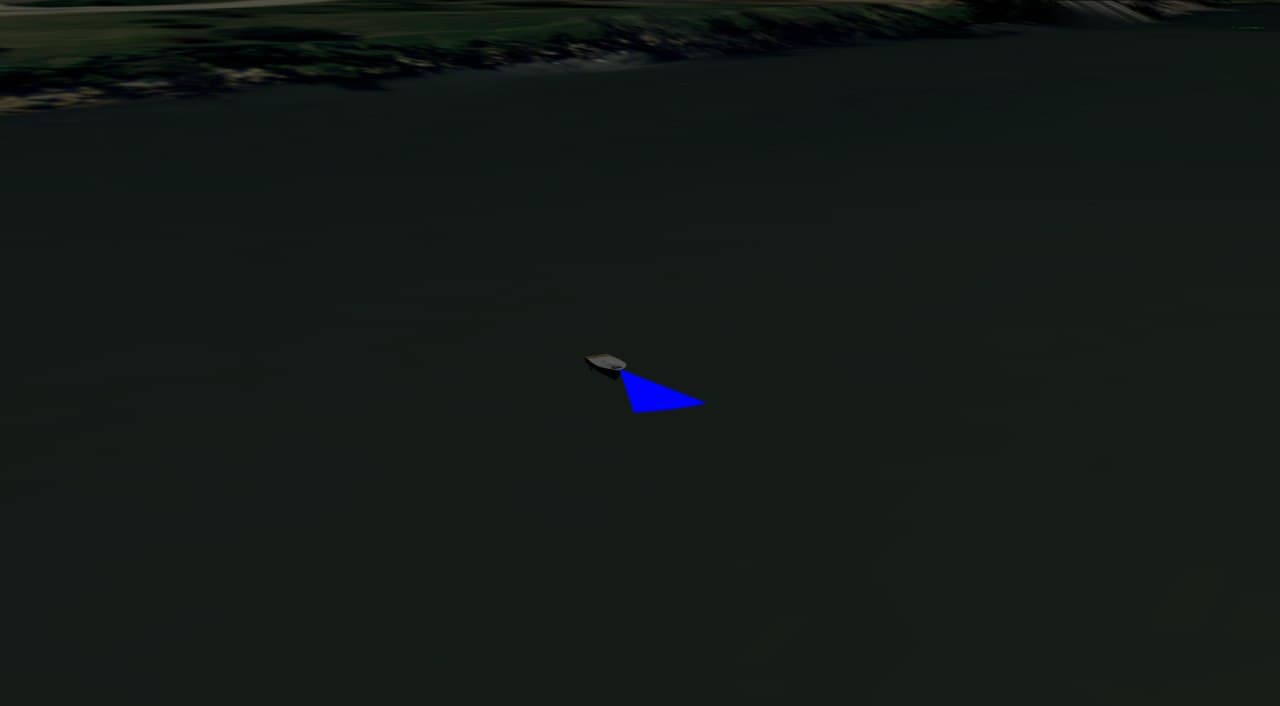
\includegraphics[width=0.8\linewidth]{sonar_boot.jpg}
	\caption{USV, Messwerte des Sonars in blau}
	\label{sonar}
\end{figure}

Die Simulationsumgebung kann man unter \url{https://github.com/uzl-usv/usv_sim_lsa} finden und downloaden. Unser Szenario startet man mit den Befehlen:
\begin{itemize}
	\item \texttt{catkin\_make\_isolated --install}
	\item \texttt{source install\_isolated/setup.bash}
	\item \texttt{roslaunch usv\_sim rescue\_robotics\_boat\_scenario1.launch parse:=true}
	\item \texttt{roslaunch usv\_sim rescue\_robotics\_boat\_scenario1.launch parse:=false}
	\item \texttt{rosservice call /gazebo/unpause\_physics "{}"}
\end{itemize}
In dem Projekt \url{https://github.com/uzl-usv/usv} ist das implementierte Verhalten des Bootes, also das Abfahren des Gewässers mit gleichzeitiger Aufnahme der Wassertiefe, zu finden. Dieses Verhalten startet man durch den Befehl:

\begin{itemize} \label{launch}
	\item \texttt{roslaunch boot usv.launch params\_file:=<path\_to\_param\_file.yaml>}
\end{itemize}

\lstinputlisting[label={params}, caption={Parameter für den Start eines Szenarios}, language=yaml]{../versuch1.yaml}

Davor müssen bestimmte Parameter in einer yaml-Datei gesetzt werden wie in Listing \ref{params}. Diese Parameter haben folgende Bedeutungen:
\begin{itemize}
	\item \texttt{origin/lat}, \texttt{origin/lon}: die GPS-Koordinaten der unteren linken Ecke der angegebenen Karte
	\item \texttt{home/lat}, \texttt{home/lon}: die GPS-Koordinaten, zu denen im Falle eines Problems oder nach erfolgreichem Beenden der Aufgabe zurückgekehrt werden soll
	\item \texttt{measurements/file\_name}: Pfad zu der Datei, in der die Messungen gespeichert werden sollen
	\item \texttt{measurements/start/lat}, \texttt{measurements/start/lon}: der Startpunkt der Messungen (dies muss der süd-westlichste Punkt sein, an dem eine Messung erfolgen soll)
	\item \texttt{measurements/width}, \texttt{measurements/height}: die Höhe und Breite des zu erfassenden Gebietes
	\item \texttt{measurements/dist}: das Intervall in Metern, in dem Messdaten aufgenommen werden sollen
\end{itemize}
Der Pfad zu dieser yaml-Datei muss der launch-Datei übergeben werden. Nach der Simulation kann man die Ergebnisse der Messungen dann in den angegebenen Dateien finden.
Wir haben das Szenario mit verschiedenen Einstellungen gestartet:

\begin{center}
\begin{tabular}[t]{|c|c| c| c| c|}
	\hline
	& & \multicolumn{3}{c|}{measurements}\\
	Versuch&origin&start& & \\
	Nummer	&lat, lon 			& lat, lon 			& height x width & dist\\
	\hline
	1	&-30.048638,-51.236690		&-30.047311,-51.234663		&15 x 15	&5\\
	\hline
	2	&-30.048638,-51.236690 		& -30.047407,-51.234420 	&20 x 16	&4\\
	\hline
	3	& -30.048638, -51.236690	& -30.047358, -51.233064	& 20 x 16 	&4\\
	\hline
	4	& -30.048638, -51.236690	& -30.047407, -51.234420	& 20 x 15 	&2.5 \\
	\hline
	5,6	&-30.048638,-51.236690		&-30.047311,-51.234663		&15 x 15	&5\\
	\hline
	7	&-30.048638,-51.236690		& -30.047407, -51.234420	& 9 x 15	& 2\\
	\hline
\end{tabular}
\end{center}

\subsection{Versuch Nummer 1: freie Fläche}
In Versuch Nummer 1 sollte eine freie Fläche von $225m^2$ abgefahren werden. In einem Abstand von $5m$ sollten Messwerte aufgenommen werden. Der abzufahrende Bereich (rotes Rechteck in Abbildung \ref{Versuch1}) wurde im Versuch komplett abgefahren und danach ist das Boot zu den gewünschten Koordinaten zurückgekehrt. Messwerte wurden beim Fahren ebenfalls in den angegebenen Abständen erzeugt (s. Abbildung \ref{Versuch1}).

\begin{figure}[H]
	\centering
	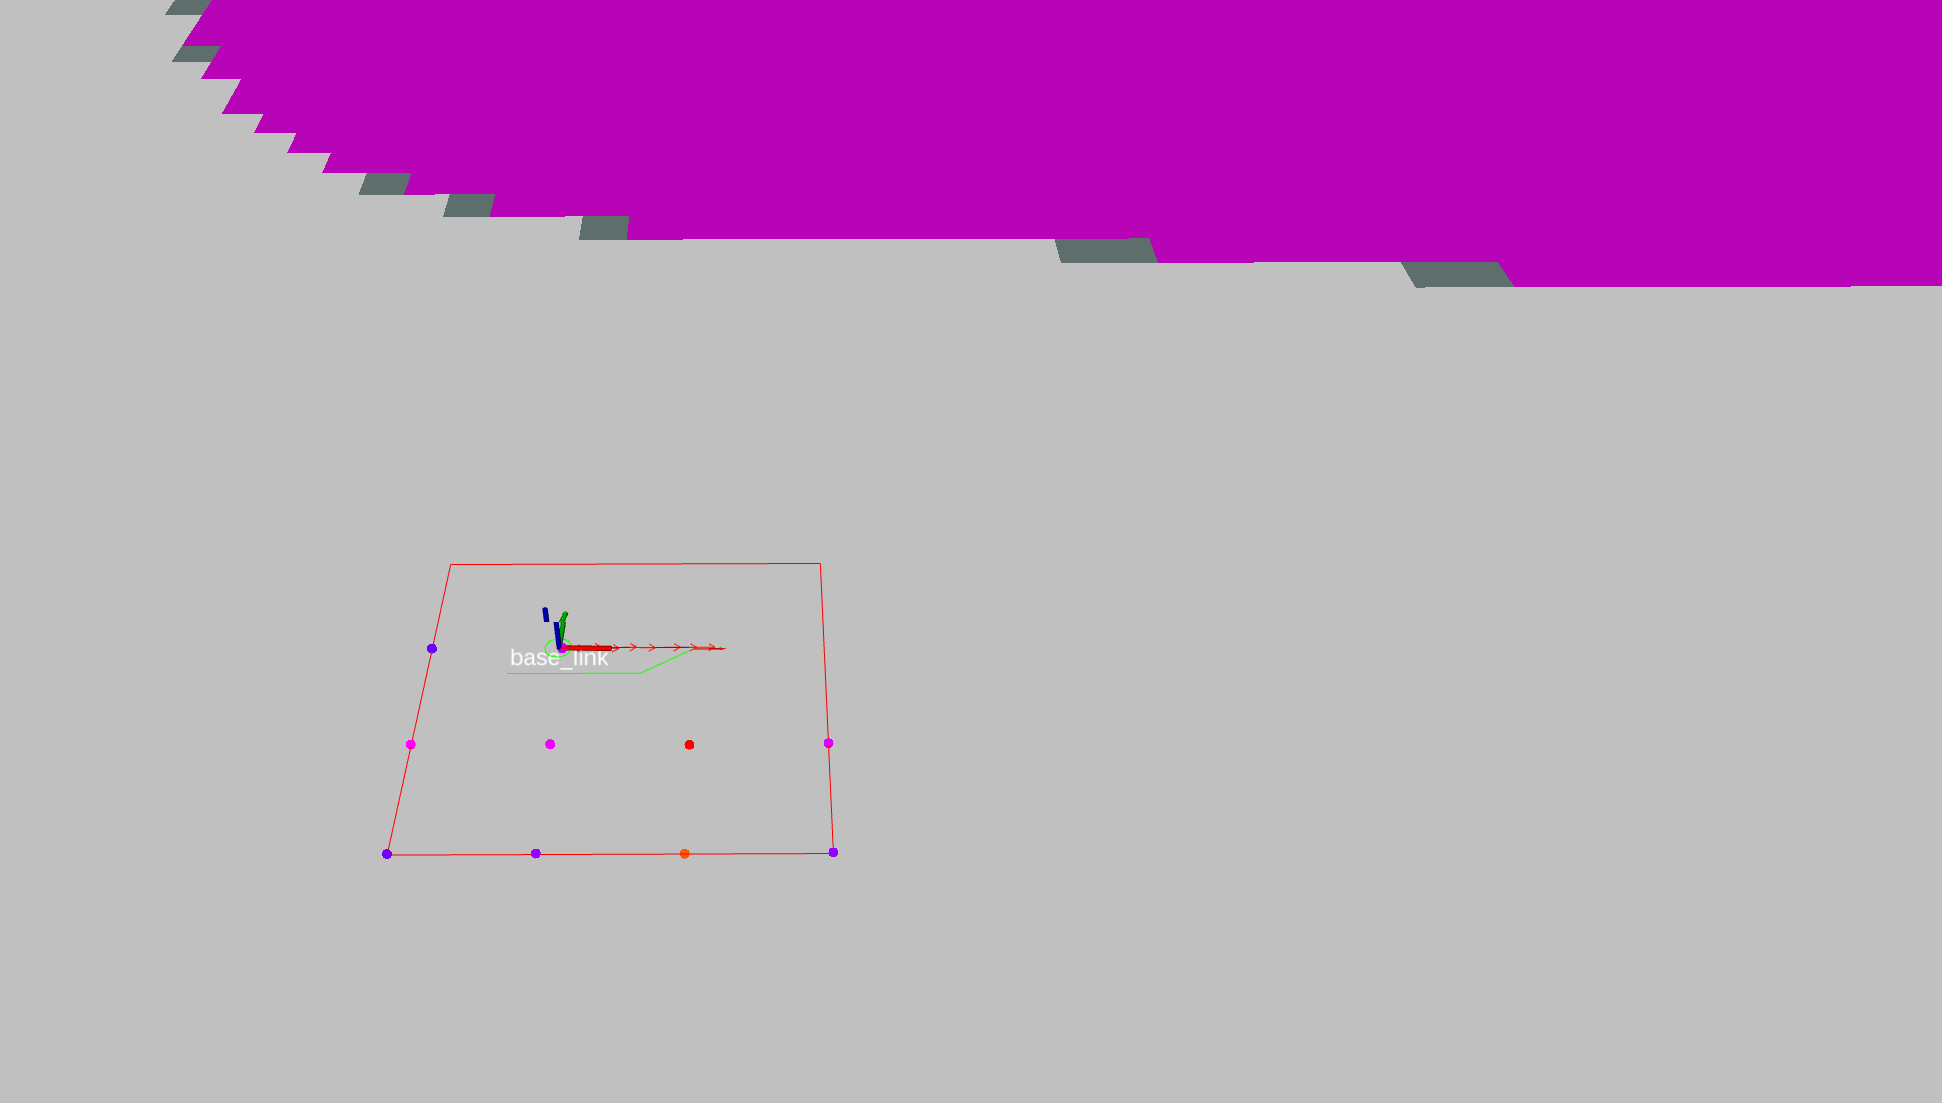
\includegraphics[width=0.8\linewidth]{versuch1.png}
	\caption{Versuch Nummer 1: freie Fläche}
	\label{Versuch1}
\end{figure}

\subsection{Versuch Nummer 2: unerwartete Hindernisse}
In Versuch Nummer 2 sollte eine Fläche abgefahren werden, die $20mx16m$ umfasst (s. rotes Rechteck in Abbildung \ref{Versuch2}). Messwerte sollten in einem Abstand von $4m$ aufgenommen werden. Darüber hinaus befanden sich in dem Gebiet Bojen, deren Anwesenheit dem Boot nicht bekannt war. Allen Bojen wurde während des Tests erfolgreich ausgewichen. Ein Beispiel ist in Abbildung \ref{Versuch2} zu sehen.

\begin{figure}[H]
	\centering
	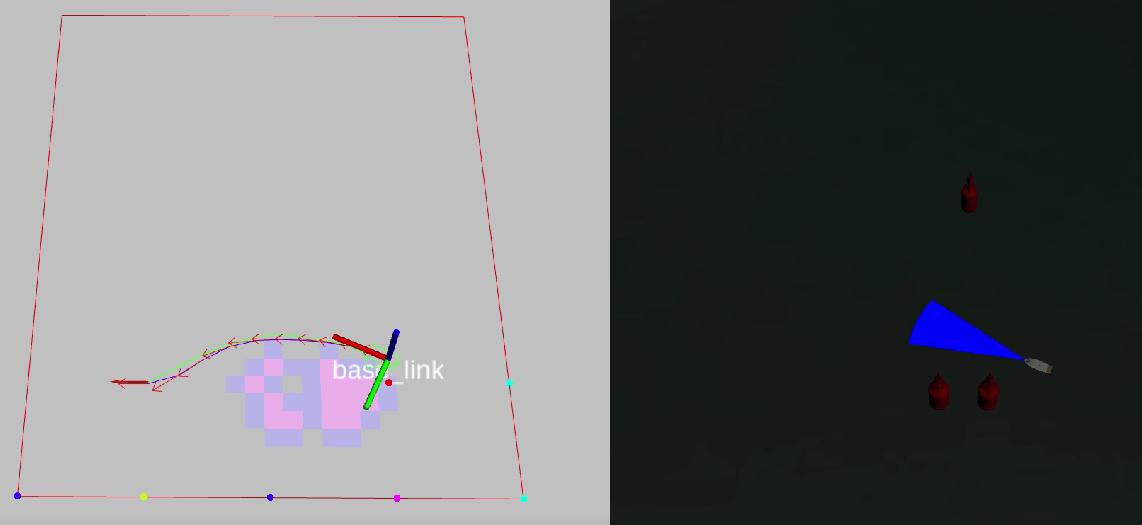
\includegraphics[width=0.8\linewidth]{versuch2.png}
	\caption{Versuch Nummer 2: unerwartete Hindernisse}
	\label{Versuch2}
\end{figure}

\subsection{Versuch Nummer 3: Fläche mit unerreichbaren Regionen (erwartet)}
In Versuch Nummer 3 sollte eine Fläche von $20mx16m$ abgefahren werden und dabei in Abständen von $4m$ Messwerte aufgenommen werden. Außerdem waren Teile des Gebietes unbefahrbare Regionen und auch als solche im Occupancy Grid gespeichert. Zielpunkte, die in nicht befahrbaren Regionen lagen, wurden im Laufe des Tests erfolgreich übersprungen (s. Abbildung \ref{Versuch3}).

\begin{figure}[H]
	\centering
	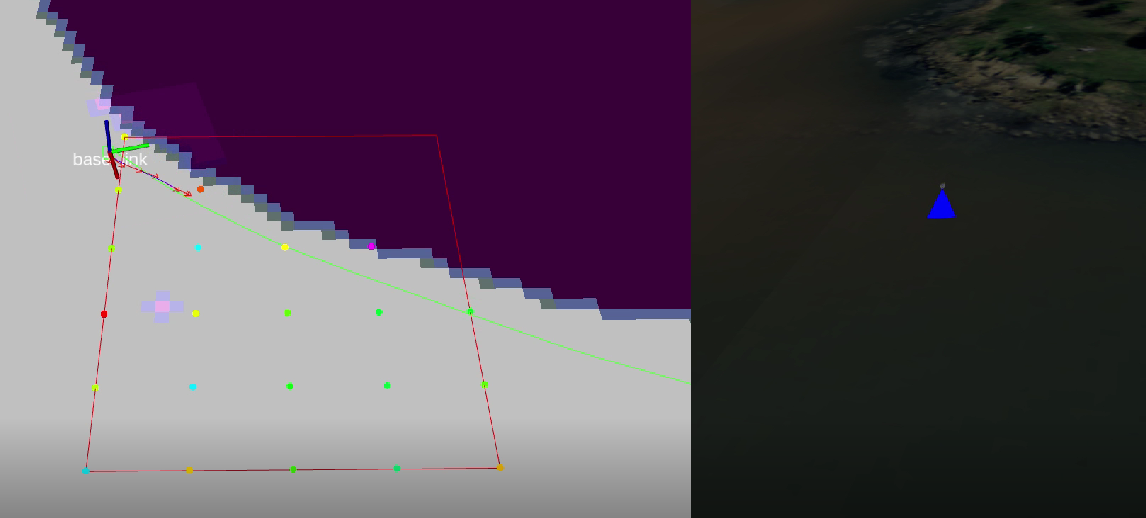
\includegraphics[width=0.8\linewidth]{versuch3.png}
	\caption{Versuch Nummer 3: unbefahrbare Region (erwartet)}
	\label{Versuch3}
\end{figure}

\subsection{Versuch Nummer 4: Fläche mit unerreichbaren Regionen (unerwartet)}
In Versuch Nummer 4 sollte eine Fläche von $20mx15m$ abgefahren werden und dabei in Abständen von $2.5m$ Messwerte aufgenommen werden. Außerdem waren Teile des Gebietes unbefahrbare Regionen, aber nicht als solche im Occupancy Grid gespeichert. Das Hindernis wurde vom Boot immer erkannt und umfahren. Zielpunkte, die nicht anfahrbar waren, weil sie im Hindernis lagen, wurden vom Boot übersprungen. Danach fuhr das Boot wie geplant mit der Messung fort (s. Abbildung \ref{Versuch4}).

\begin{figure}[H]
	\centering
	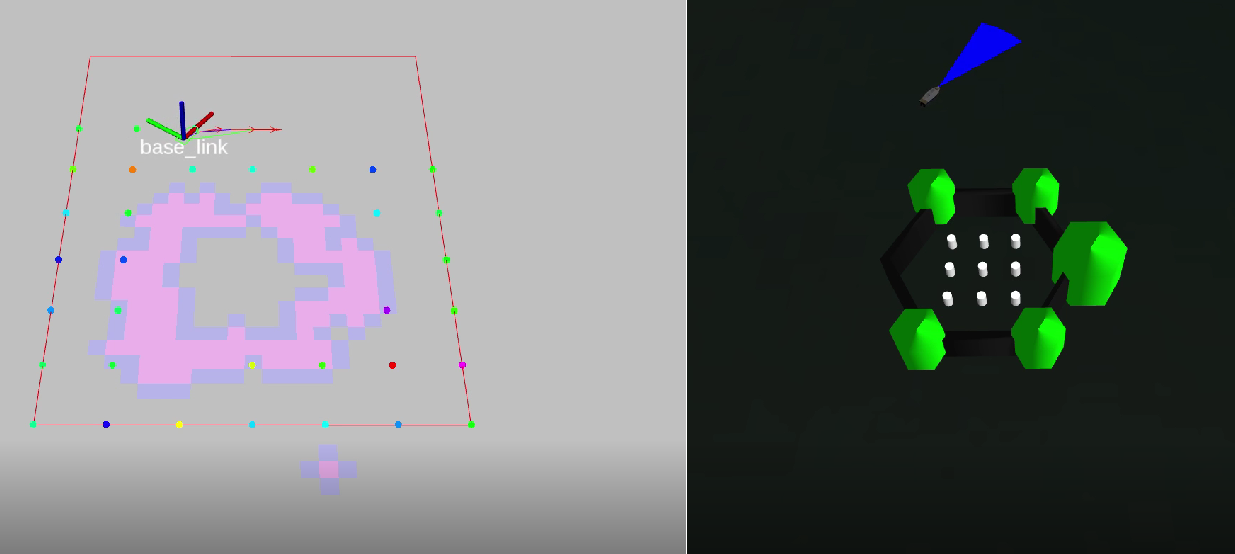
\includegraphics[width=0.8\linewidth]{versuch4.png}
	\caption{Versuch Nummer 4: unbefahrbare Region (unerwartet)}
	\label{Versuch4}
\end{figure}

\subsection{Versuch Nummer 5, 6: Batteriestand gering, Wasser im Boot}
In Versuchen Nummer 5 und 6 sollte eine Fläche von $15mx15m$ abgefahren werden und dabei in Abständen von $5m$ Messwerte aufgenommen werden. Während des Fahrens sollte der Batteriestand unter 20\% fallen, bzw. der Wassersensor Wasser im Boot feststellen, so dass das Boot direkt "nach Hause" zurückkehren sollte. In beiden Fällen wurde das Verhalten korrekt ausgeführt.\\

\subsection{Versuch 7: Abbruch und Neustart der Messung}
In Versuchen Nummer 7 sollte eine Fläche von $9mx15m$ abgefahren und dabei in Abständen von $2m$ Messwerte aufgenommen werden. Nach 11 Messpunkten wurde die Messung einmal abgebrochen und dann neu gestartet. Wie in Abbildung \ref{Versuch7} zu sehen, wurden dann erst wieder Messwerte ab Punkt 12 aufgenommen. Da die Höhe und Breite des Bereichs nicht ganzzahlig durch die  Messabstände teilbar waren, wurden Bereiche an den Rändern ausgelassen.

\begin{figure}[H]
	\centering
	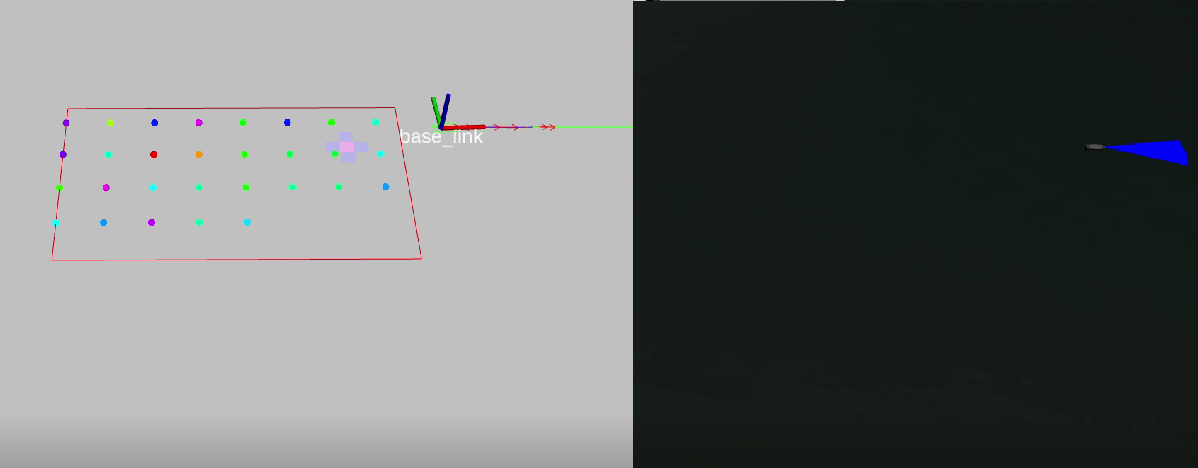
\includegraphics[width=0.8\linewidth]{versuch7.png}
	\caption{Versuch Nummer 7: Neustart nach Abbruch}
	\label{Versuch7}
\end{figure}

\subsection{Zusammenfassung}
Die Zielpunkte wurden in allen Versuchen richtig gesetzt und der Bereich damit korrekt abgefahren. Dabei wurden Orte, die sich in einem (erwartet oder unerwartet) unbefahrbaren Bereich befanden, übersprungen und Hindernissen ausgewichen.\\
Bei Abbruch der Messung konnte der Versuch später erfolgreich fortgeführt werden und bei Problemen oder nach Beenden der Messungen fuhr das Boot zu den dafür vorher festgelegten Koordinaten.\\
Die Messung der Wassertiefe konnte im Simulator leider nur bedingt getestet werden, da die Wasseroberfläche als Hindernis wahrgenommen wird. Deshalb wurde dort wie erwartet immer Werte zurückgegeben, die um den Minimalwert des Sensors schwankten. Die Messwerte und ihre Koordinaten wurden nach allen Versuchen automatisch in einer Datei gespeichert.


\section{Fazit} \label{fazit}
Unser am Anfang gestecktes Ziel, das USV durch Software zu ergänzen, die ein autonomes Befahren eines Gewässers und die gleichzeitige Aufnahme von Messwerten ermöglicht, wurde im Laufe der Projektarbeit erreicht. Auch die Simulation des Bootes ist grundsätzlich funktionsfähig. Eine Ausnahme bildet die Messung der Wassertiefe, welche bislang nicht gemessen werden kann, da der Ultraschallsensor die Wasseroberfläche als Hindernis wahrnimmt. Außerdem verfügt das Boot noch über weitere Sensoren, die wir im Modell nicht beachtet haben, da wir sie für unseren Anwendungsfall nicht benötigten. Diese sollten aber relativ unproblematisch zu unserem Modell hinzugefügt werden können, so dass unser Modell auch für weitere Projekte eine gute Grundlage bilden sollte.\\
Die Menge der Anwendungsfälle, in denen das Boot genutzt werden kann, ist bisher begrenzt. Die Messung der Wassertiefe könnte dabei helfen, vermisste Personen im Wasser zu lokalisieren. Andere Problemstellungen, wie zum Beispiel das Erkennen von Deichbrüchen und Verschmutzungen, können bis jetzt nicht abgedeckt werden. Aber auch für diese noch zu implementierenden Anwendungsfälle liefert das bereits erreichte autonome Befahren des Gewässers sicher eine gute Grundlage, da zuverlässig Hindernissen ausgewichen werden kann und das Boot im Problemfall nicht verloren geht, sondern zu bestimmten Koordinaten fährt.

\bibliography{bericht}{}
\bibliographystyle{IEEEtran}

\end{document}
